\documentclass{article}
\usepackage[margin=1in]{geometry}
\usepackage{graphicx}
\usepackage{xcolor}
\usepackage{float}
\usepackage{amsmath}
\graphicspath{{..} {./images}}

\renewcommand{\contentsname}{\vspace*{-2\baselineskip}}

\begin{document}
\begin{titlepage}
	\centering
	{\huge Lab 1 - Introduction to Software-Defined Radio}\\[0.25 in]
	
\includegraphics[width=0.6\textwidth]{ua_logo.png}\\[0.25 in]
	{\large \textbf{ECE 531 - Software Defined Radio\\[0.25 in]
	Spring 2025\\[0.25 in]}}
	{\large Owen Sowatzke, osowatzke@arizona.edu\\[0.05 in]
	Department of Electrical \& Computer Engineering\\[0.05 in]
	University of Arizona, Tucson, AZ 85721\\[0.5 in]}
	\textcolor{blue}{
	\noindent\hrulefill
	\tableofcontents
	\noindent\hrulefill
	}
\end{titlepage}

\setlength{\parindent}{0pt}

\section{Introduction}
%Introduction to the laboratory experiment, including a brief description of the objectives and goals.

This laboratory experiment provides a review of digital signal processing, while introducing SDR flowgraphs and simulations in GNU radio. Topics reviewed include sampling rates, complex sampling, interpolation, decimation, and noise analysis. To investigate these topics we perform multiple experiments - each with its own GNU flowchart. The lab report that follows is divided into two primary sections. One presents the procedure for each experiment, and the other provides the results of each experiment.

\section{Procedure}
% Detailed explanation of the laboratory experiment, including the design, implementation, and testing of the system.

% In this lab, we investigate the effects of sampling rates on a sinusoid signal. We, then, investigate how complex sampling differs from real sampling. Next, we observe the spectrum of the sinusoid, while varying its frequency. Then, we examine the effects of I/Q imbalance on a complex-sampled signal.

In this section, we provide the procedures for each of the performed experiments. These experiments include sampling rates, complex sampling, frequency observations, I/Q imbalance, adding noise, and interpolation/decimation. Most of these experiments can be easily matched to their respective review topics. However, the linkage to the frequency observations and I/Q imbalance experiments is not as apparent. These additionally experiments highlight sampling subtopics. The frequency observations experiment, specifically, investigates aliasing when performing real and complex sampling. The I/Q imbalance experiment highlights the effects of gain and phase imbalance in the I/Q paths when performing complex sampling.

\subsection{Sampling Rates \label{subsection::sampling_rates}}

In the first experiment, we examine the effects of sampling rate. To perform this experiment, we construct the GNU radio companion (GRC) flowchart shown in Figure \ref{fig::sampling_rates_experiment}. We, then, use the "Time" and "Frequency" tabs of the QT GUI to examine the sampled signal.

\begin{figure}[H]
	\centerline{\fbox{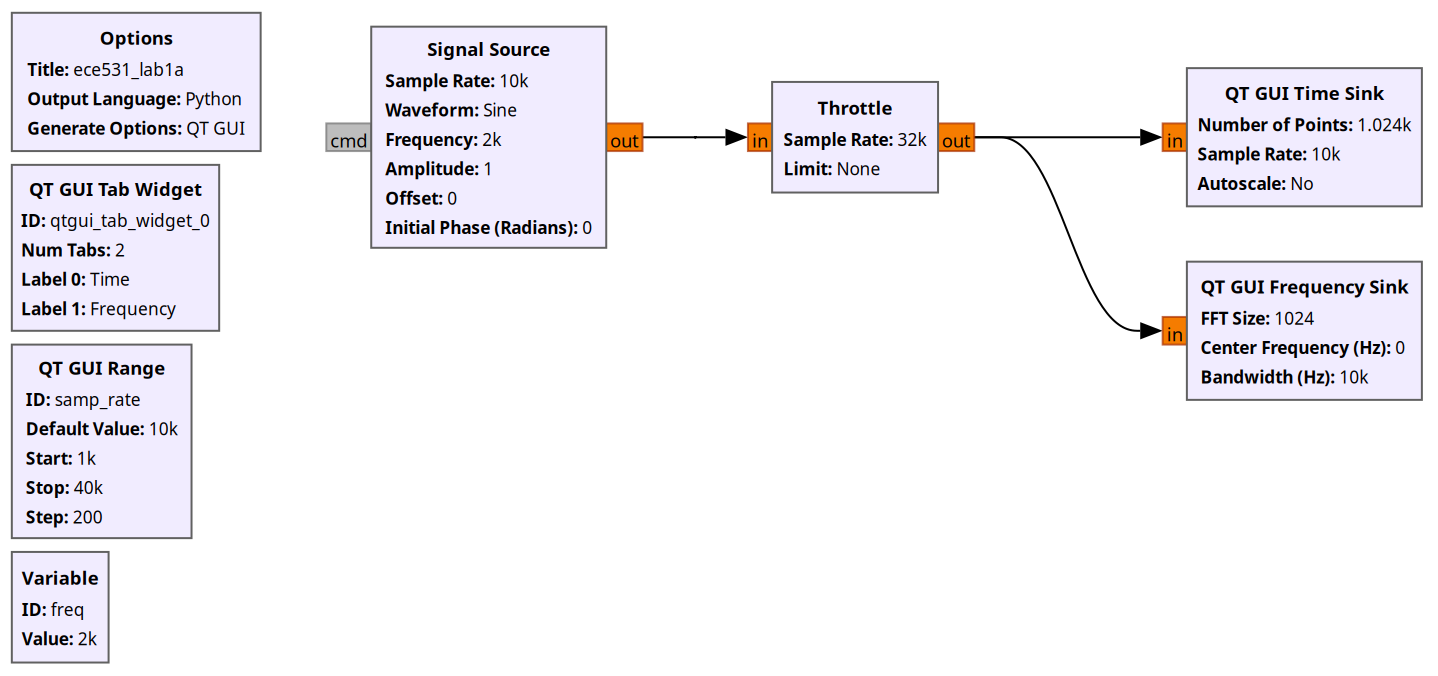
\includegraphics[width=0.7\textwidth]{sampling_rates_experiment.png}}}
	\caption{Setup for Sampling Rate Experiment}
	\label{fig::sampling_rates_experiment}
\end{figure}

We start by examining the signal when it is sampled at the 10 kHz default sample rate. We qualitatively analyze the time-domain signal by comparing it to an ideal sinusoid. We, then, measure the frequency of the signal. Next, we increase the sample rate to 40 kHz and compare the updated time and frequency plots to the previously collected data. Finally, we decrease the sample rate to 3.5 kHz and examine the frequency of the sampled signal.

\subsection{Complex Sampling \label{subsection::complex_sampling}}

In this experiment, we examine how complex sampling differs from real sampling. To perform our analysis, we modify the data types of the blocks in the GRC flowchart shown in Figure \ref{fig::sampling_rates_experiment}. The updated blocks use a "Complex Float 32" data type instead of a "Float 32" data type. Figure \ref{fig::complex_sampling_experiment} shows the updated block diagram. Note that the port colors have changed from orange to blue to reflect the change in data type.

\begin{figure}[H]
	\centerline{\fbox{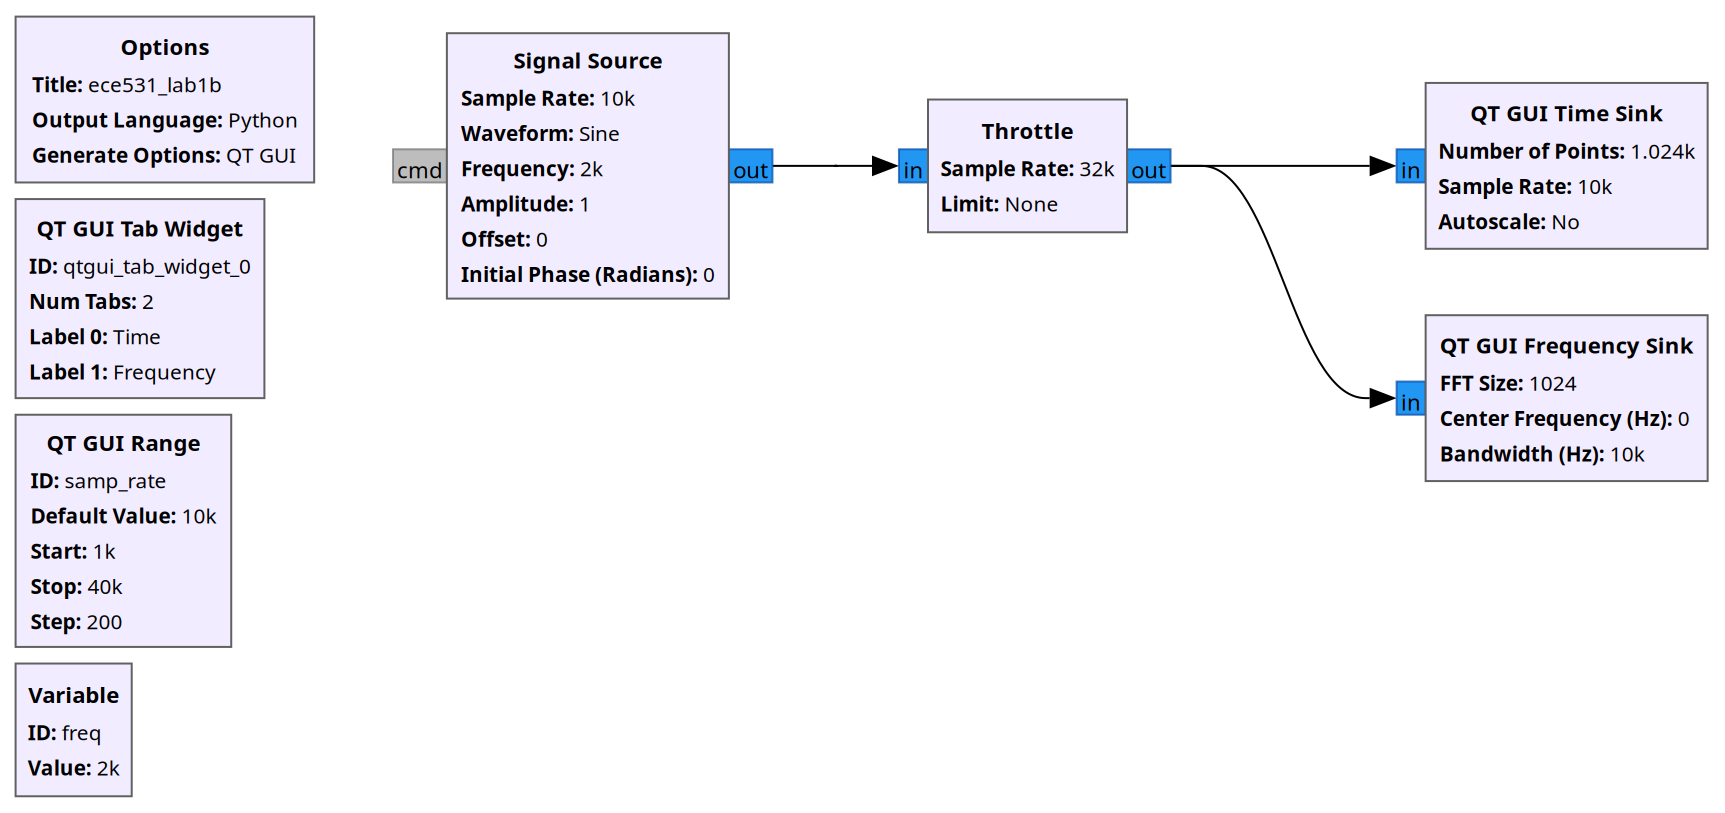
\includegraphics[width=0.7\textwidth]{complex_sampling_experiment.png}}}
	\caption{Setup for Complex Sampling Experiment}
	\label{fig::complex_sampling_experiment}
\end{figure}

Using the updated block diagram, we compare the updated frequency response to the frequency response collected in subsection \ref{subsection::sampling_rates}, noting what happens to the positive and negative frequency components. We, then, investigate the time-domain signals and measure the phase between them. Next, we examine the signal amplitude on each channel while varying the sampling frequency from 10kHz to 40kHz. At the 40kHz sampling rate, we measure the frequency peak. Then, we measure the frequency peak at a 4kHz sampling rate. Finally, we continue decreasing the sampling rate and explain the location of the frequency peak at each of the updated sampling rates.

\subsection{Frequency Observations}

In contrast to the previous experiments, we vary the frequency of the source in this experiment while keeping the sampling rate constant. We perform this exercise for both real and complex data types. Through variations of the source frequency, we reinforce the results of the previous experiments.

%The experiment performed here reinforces the results of the previous sections and is performed on both real and complex-sampled data.
 
\subsubsection{Complex-sampled Flowgraph \label{subsection::frequency_observations_complex_sampling}}

The GRC flowchart for this experiment, using complex sampling, is shown in Figure \ref{fig::frequency_observations_complex_sampling}. Compared with the previous flowchart, the sinusoid frequency can now be controlled with a slider.

\begin{figure}[H]
	\centerline{\fbox{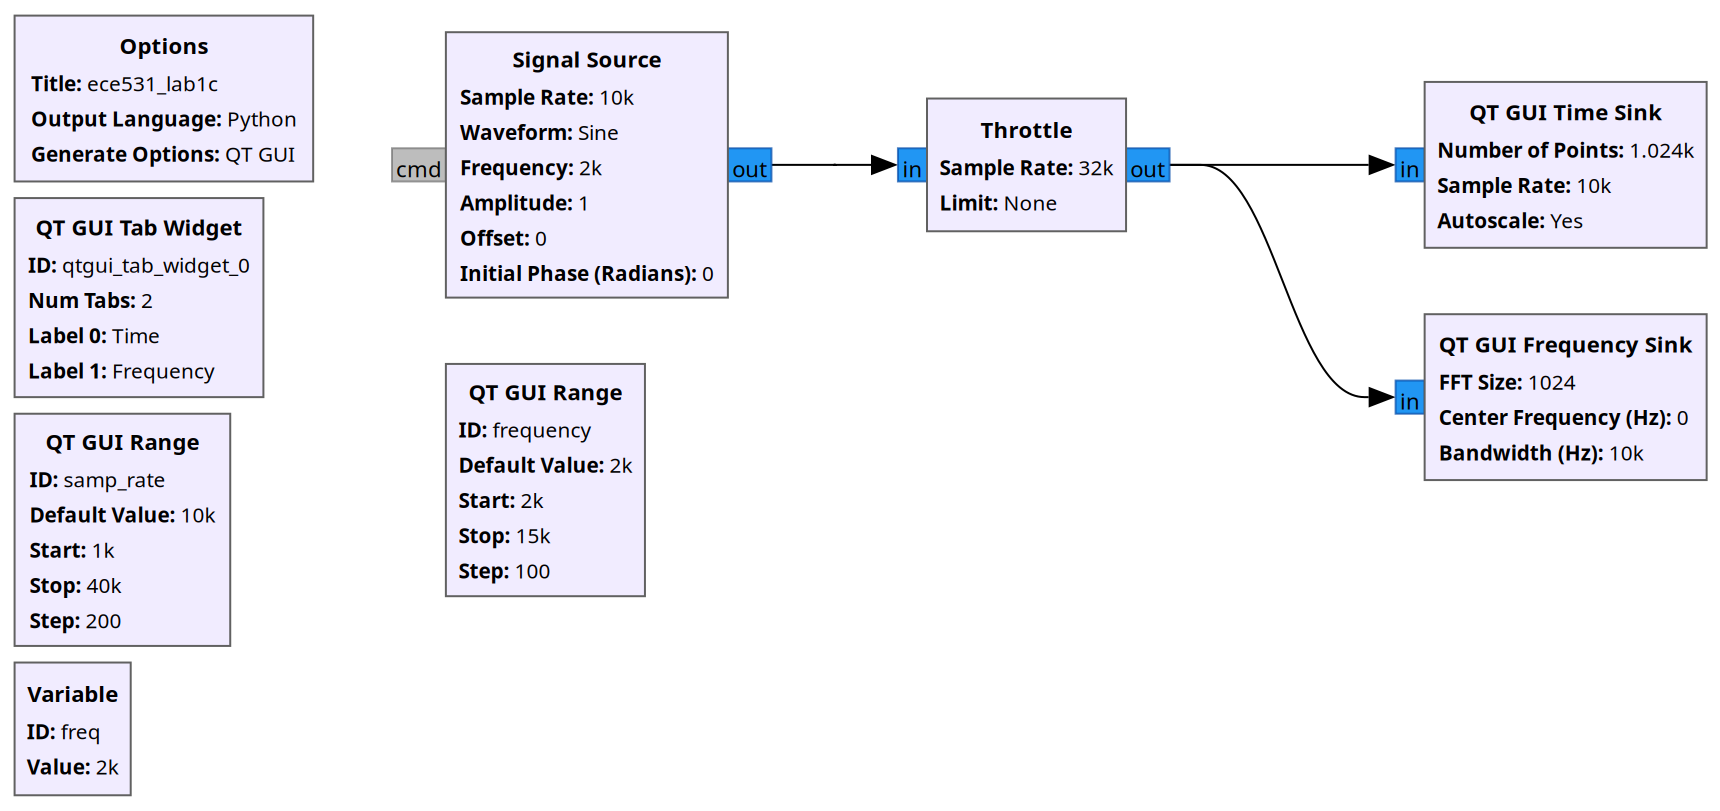
\includegraphics[width=0.7\textwidth]{frequency_observations_complex_sampling.png}}}
	\caption{Complex-sampled Frequency Observations}
	\label{fig::frequency_observations_complex_sampling}
\end{figure}

Using the updated flowchart, we vary the sinusoid frequency over its full range (from 2kHz to 15kHz), while observing the resulting spectrum. Based on the collected data, we notate any anomalies and describe why they occur. 

\subsubsection{Real-sampled Flowgraph}

We also investigate real-sampling using the flowchart shown in Figure \ref{fig::frequency_observations_real_sampling}. The flowchart is identical to the one shown in Figure \ref{fig::frequency_observations_complex_sampling} except for the data types which have been modified from "Complex Float 32" to "Float 32".

\begin{figure}[H]
	\centerline{\fbox{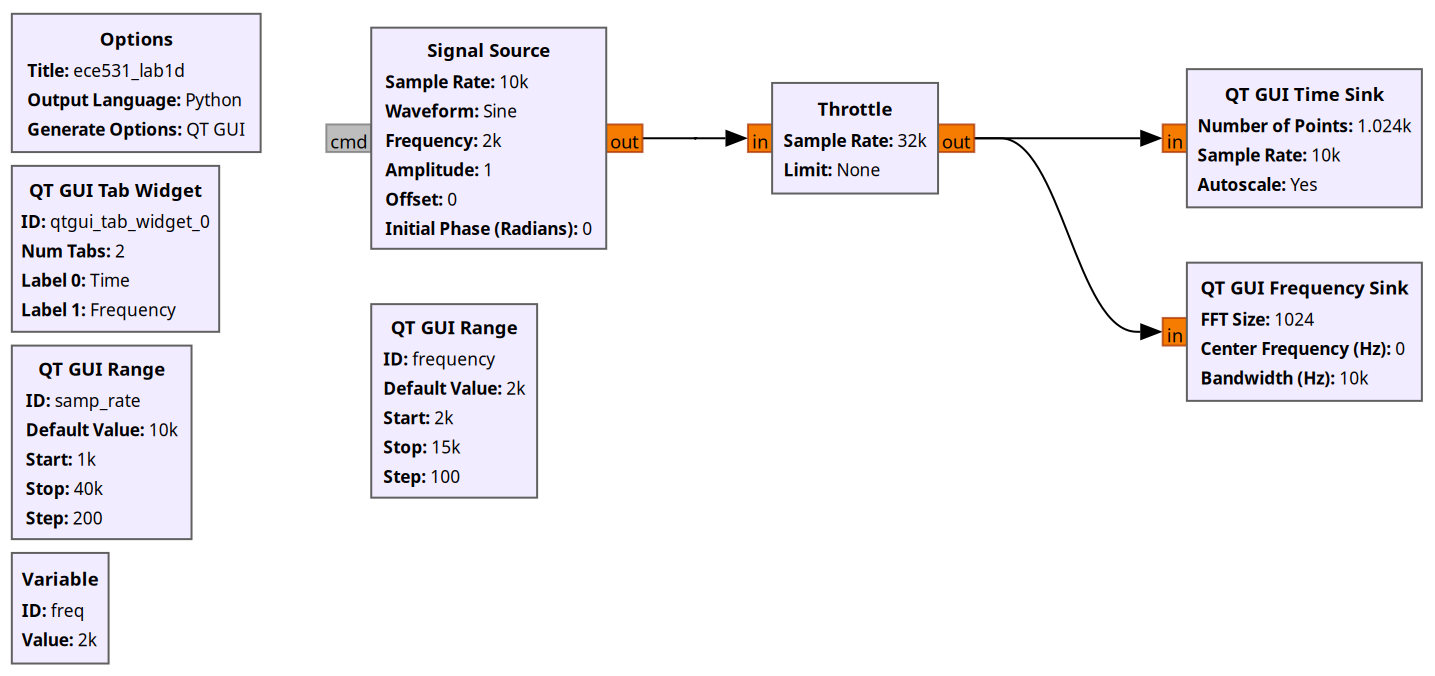
\includegraphics[width=0.7\textwidth]{frequency_observations_real_sampling.png}}}
	\caption{Real-sampled Frequency Observations}
	\label{fig::frequency_observations_real_sampling}
\end{figure}

Using the above flowchart, we vary the sinusoid frequency over its full range (from 2kHz to 15kHz). We observe the resulting spectrum and compare to the results we observed in Section \ref{subsection::frequency_observations_complex_sampling}.

\subsection{I/Q Imbalance}

In this experiment, we investigate the effect of I/Q imbalance on complex sampling. I/Q imbalance refers to a gain-phase mismatches in the I (in-phase) and Q (quadrature) paths. These gain-phase mismatches degrade the sampled signal and result in distortion. Figure \ref{fig::iq_imbalance_experiment} shows the GNU radio flowchart used to investigate I/Q imbalance.

\begin{figure}[H]
	\centerline{\fbox{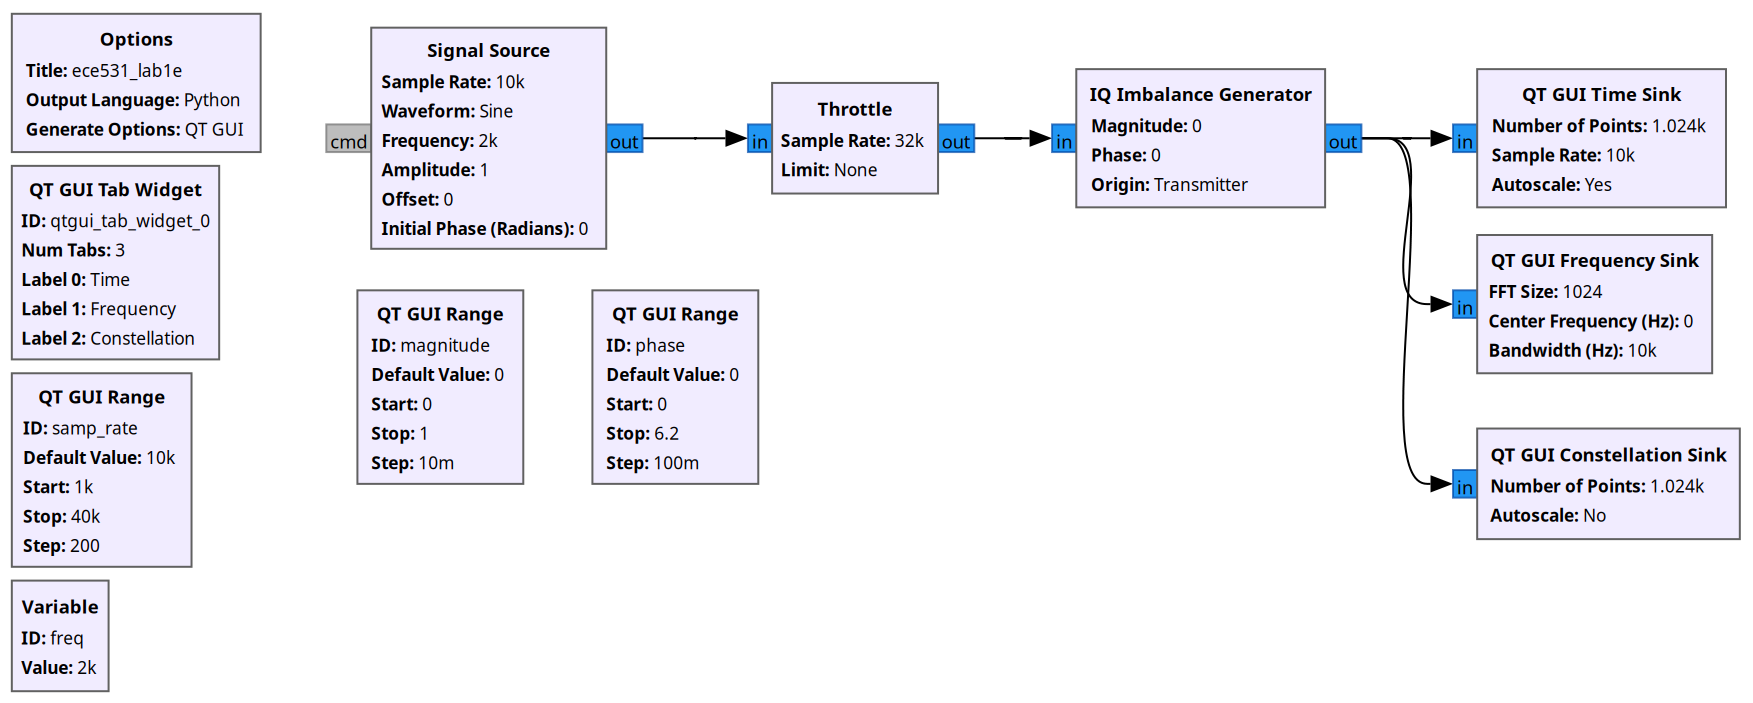
\includegraphics[width=0.7\textwidth]{iq_imbalance_experiment.png}}}
	\caption{I/Q Imbalance Experiment}
	\label{fig::iq_imbalance_experiment}
\end{figure}

With the experiment setup, we first execute with the default values (no gain and phase imbalance) and verify the results are identical to those collected previously. Next, we observe the frequency response while independently varying the gain and phase imbalances - notating what occurs and why. Then, we observe the captured constellation while independently varying the frequency, magnitude, and phase. For each variable that we vary, we log what happens to the received constellation.  

\subsection{Adding Noise}

In this experiment, we build off the flowchart shown in Figure \ref{fig::complex_sampling_experiment} by adding noise to the sinusoidal signal. The resulting flowchart is shown in Figure \ref{fig::noise_experiment}.

\begin{figure}[H]
	\centerline{\fbox{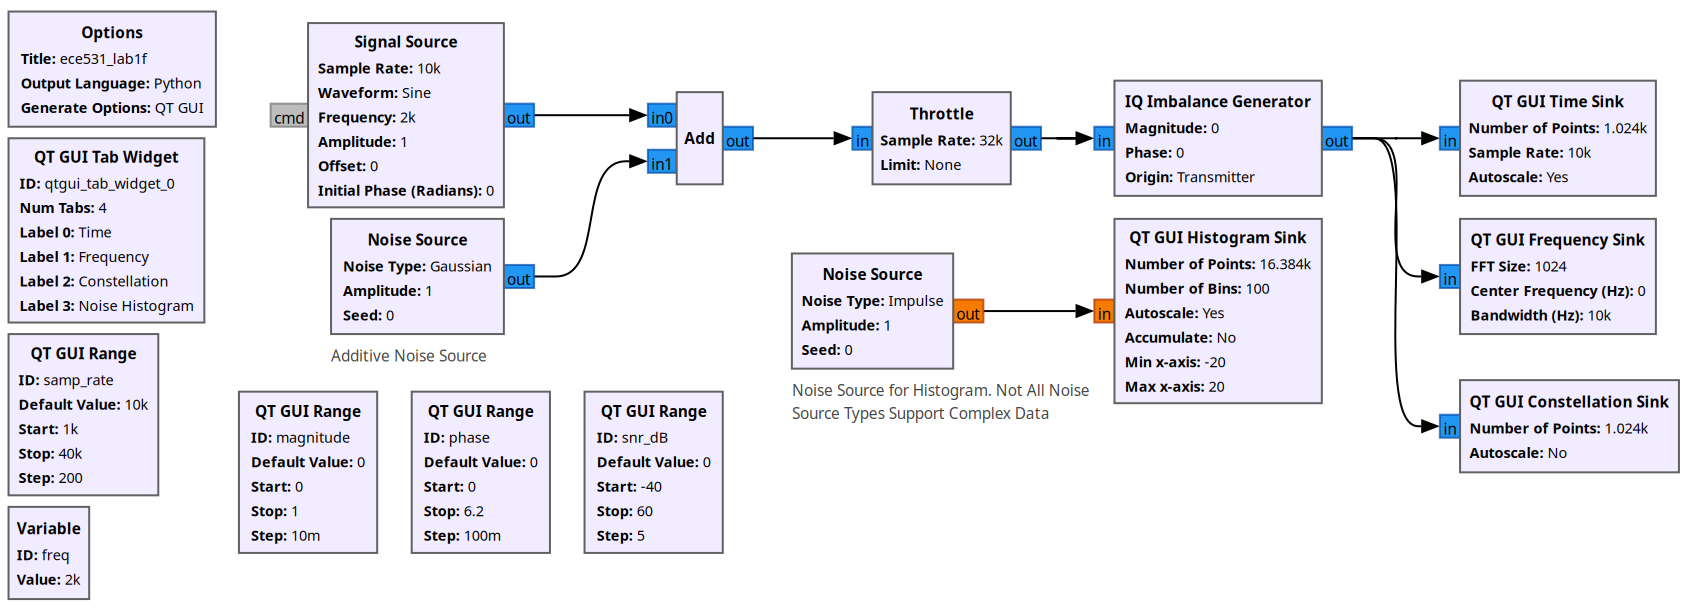
\includegraphics[width=0.7\textwidth]{noise_experiment.png}}}
	\caption{Noise Experiment}
	\label{fig::noise_experiment}
\end{figure}

Using the updated flowchart, we explore the effects of the additive noise on the time-domain signal, the frequency-domain signal, and the resulting constellation. Next, we use the histogram tab to verify the probability density function (pdf) of each noise source type. Note that the histogram tool only supports real data types. As such, we must independently examine the real and imaginary parts of the complex source. However, the laplacian and impulse noise sources only support real types, so we instead add an additional real noise source for this portion of the experiment. 

% Note that we use a separate noise source for the histogram because the laplacian and impulse noise sources do not support complex types. We 

\subsection{Interpolation and Decimation}

For the final experiment, we investigate interpolation and decimation, which are used to resample signals. The flowchart used for this analysis is given in Figure \ref{fig::interpolation_and_decimation_experiment}.

\begin{figure}[H]
	\centerline{\fbox{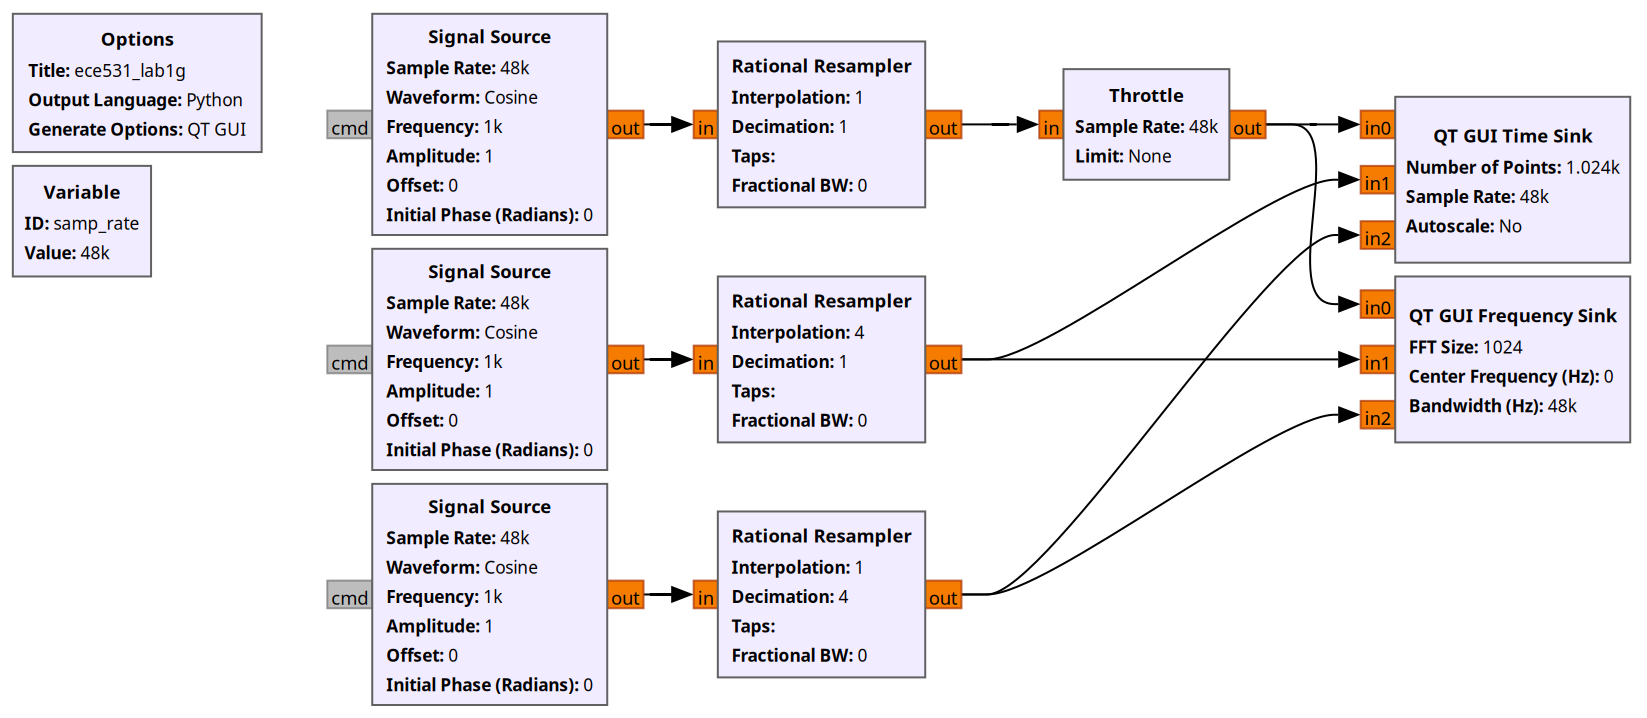
\includegraphics[width=0.7\textwidth]{interpolation_and_decimation_experiment.png}}}
	\caption{Interpolation and Decimation Experiment}
	\label{fig::interpolation_and_decimation_experiment}
\end{figure}

Using the above flowchart, we observe the time and frequency domain outputs and compare the differences between each of the resampled signals. We specifically concentrate on the differences we observe in the frequency domain and identify the relationship between each of the signals in this domain.

\section{Results}
% Results and discussion of the laboratory experiment, including captured outputs, observations, and responses to laboratory questions.

This section highlights the results from each of the experiments and provides answers to additional followup questions. The followup questions discuss the benefits of I/Q sampling, the GNU throttling block, nyquist zones, and the purpose of dither noise.

\subsection{Sampling Rates}

Using the GNU flowchart shown in Figure \ref{fig::sampling_rates_experiment}, we can view the sampled signal in the time-domain. With a 10 kHz sample rate, the resulting signal is shown in Figure \ref{fig::sampling_rates_time_domain_10k_samp_rate}.

\begin{figure}[H]
	\centerline{\fbox{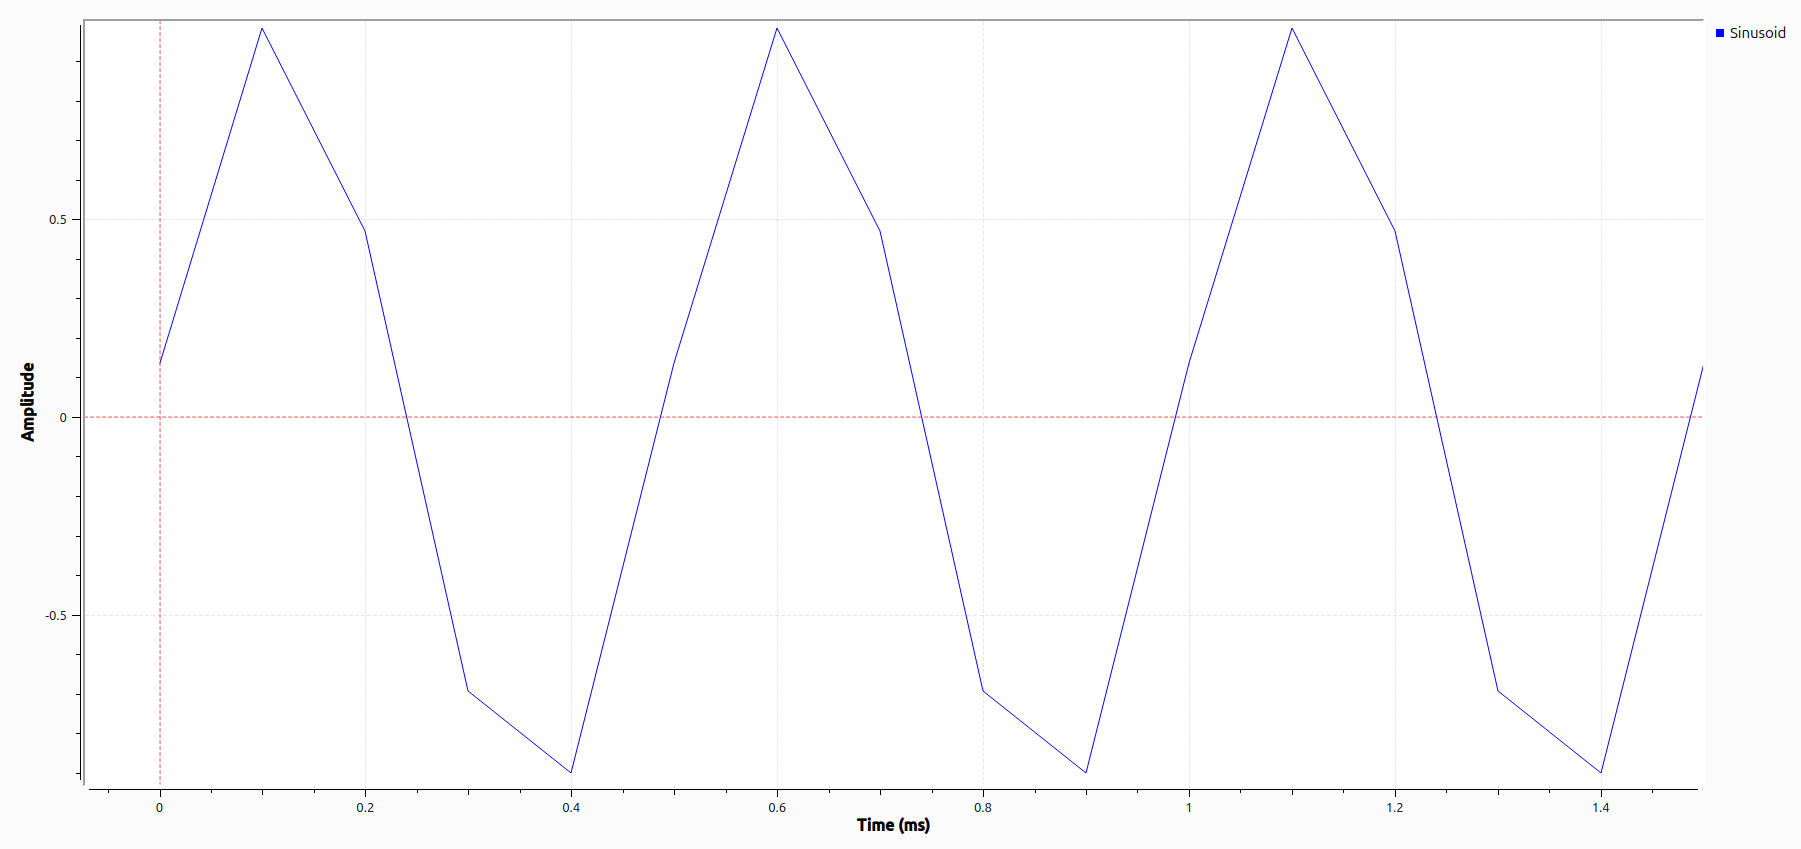
\includegraphics[width=0.7\textwidth]{sampling_rates_time_domain_10k_samp_rate.png}}}
	\caption{Time-Domain Capture of Sinusoid Sampled at 10 kHz}
	\label{fig::sampling_rates_time_domain_10k_samp_rate}
\end{figure}

Reviewing the time domain data, we see that the signal is periodic with a period of 0.5 ms, which is consistent with the 2 kHz sinusoid frequency. We also see the samples are separated by 0.1 ms, which is consistent with the 10 kHz sampling rate. Compared to a continuous time sinusoid, we note that the sampled sinusoid has many jagged edges. These edges occur because the plotting tool performs linear interpolation between samples. Even with the jagged edges, we can clearly tell that it is a sinusoid.

Figure \ref{fig::sampling_rates_freq_domain_10k_samp_rate} shows the frequency response of the sampled signal. Examining the figure, we see that the frequency response peaks at $\pm$ 2 kHz, which is consistent with the sinusoid's configured frequency.

\begin{figure}[H]
	\centerline{\fbox{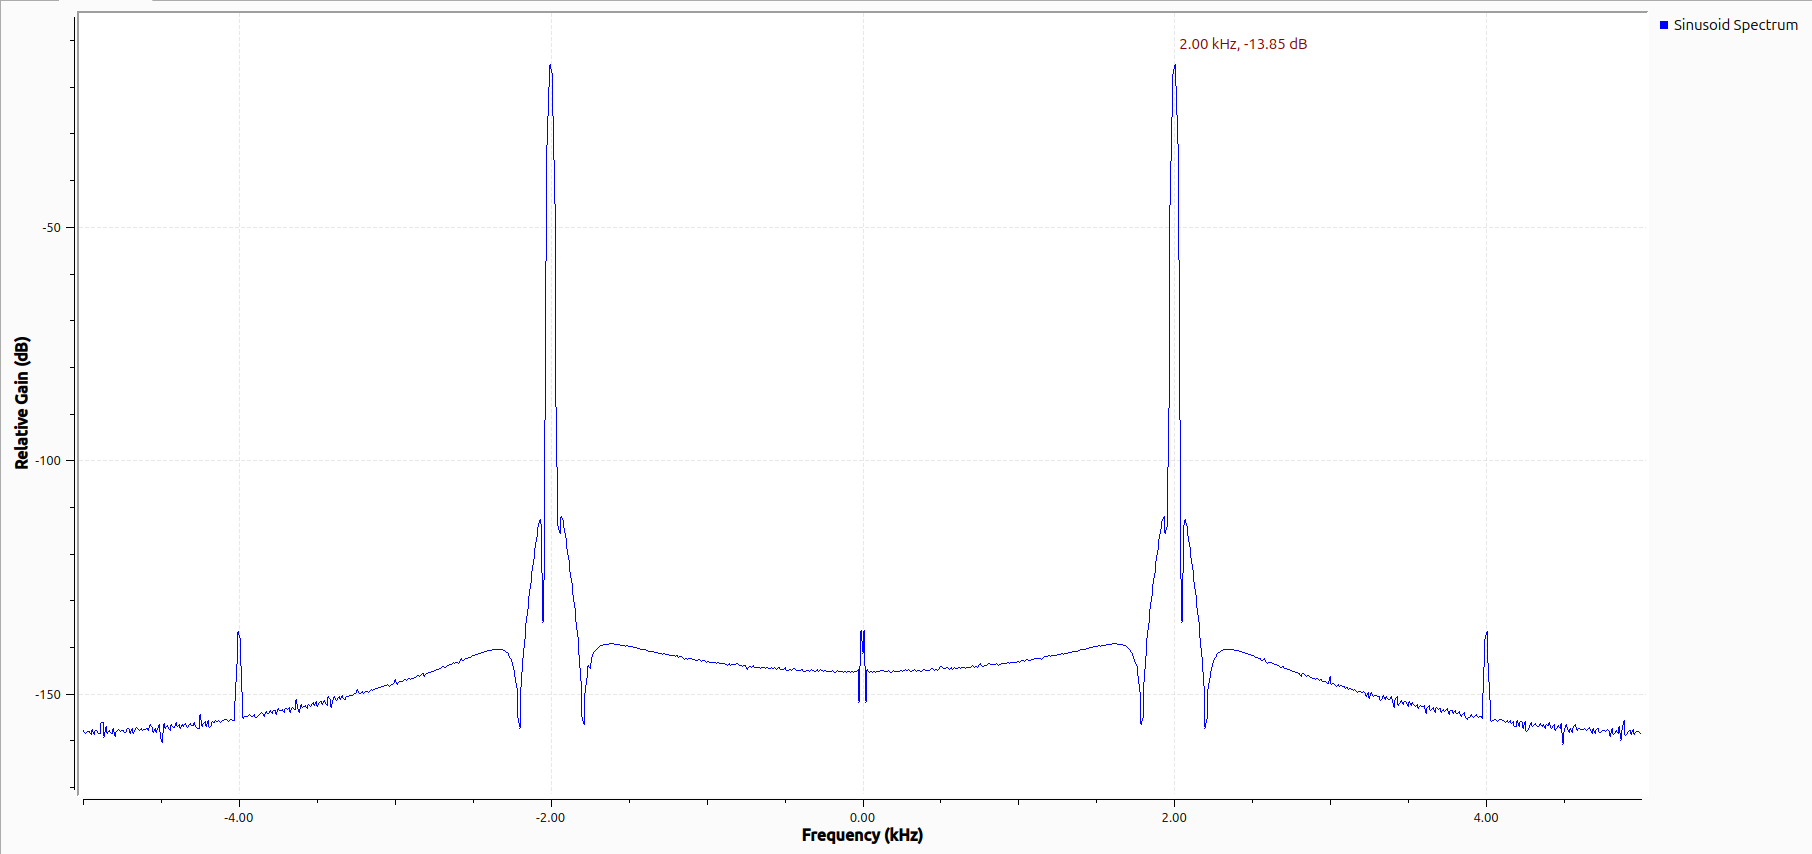
\includegraphics[width=0.7\textwidth]{sampling_rates_freq_domain_10k_samp_rate.png}}}
	\caption{Frequency Response of a Sinusoid Sampled at 10 kHz}
	\label{fig::sampling_rates_freq_domain_10k_samp_rate}
\end{figure}

Next, we examine the frequency response when the sampling rate is increased to 40 kHz. The updated frequency response is shown in Figure \ref{fig::sampling_rates_freq_domain_40k_samp_rate}. Examining the updated frequency response, we see that it peaks at $\pm$ 2 kHz, same as Figure \ref{fig::sampling_rates_freq_domain_10k_samp_rate}. The biggest difference in the resulting frequencies responses is their span. The previously collected data spanned from $\pm$ 5 kHz, while the newly collected data spans from $\pm$ 20 kHz.

\begin{figure}[H]
	\centerline{\fbox{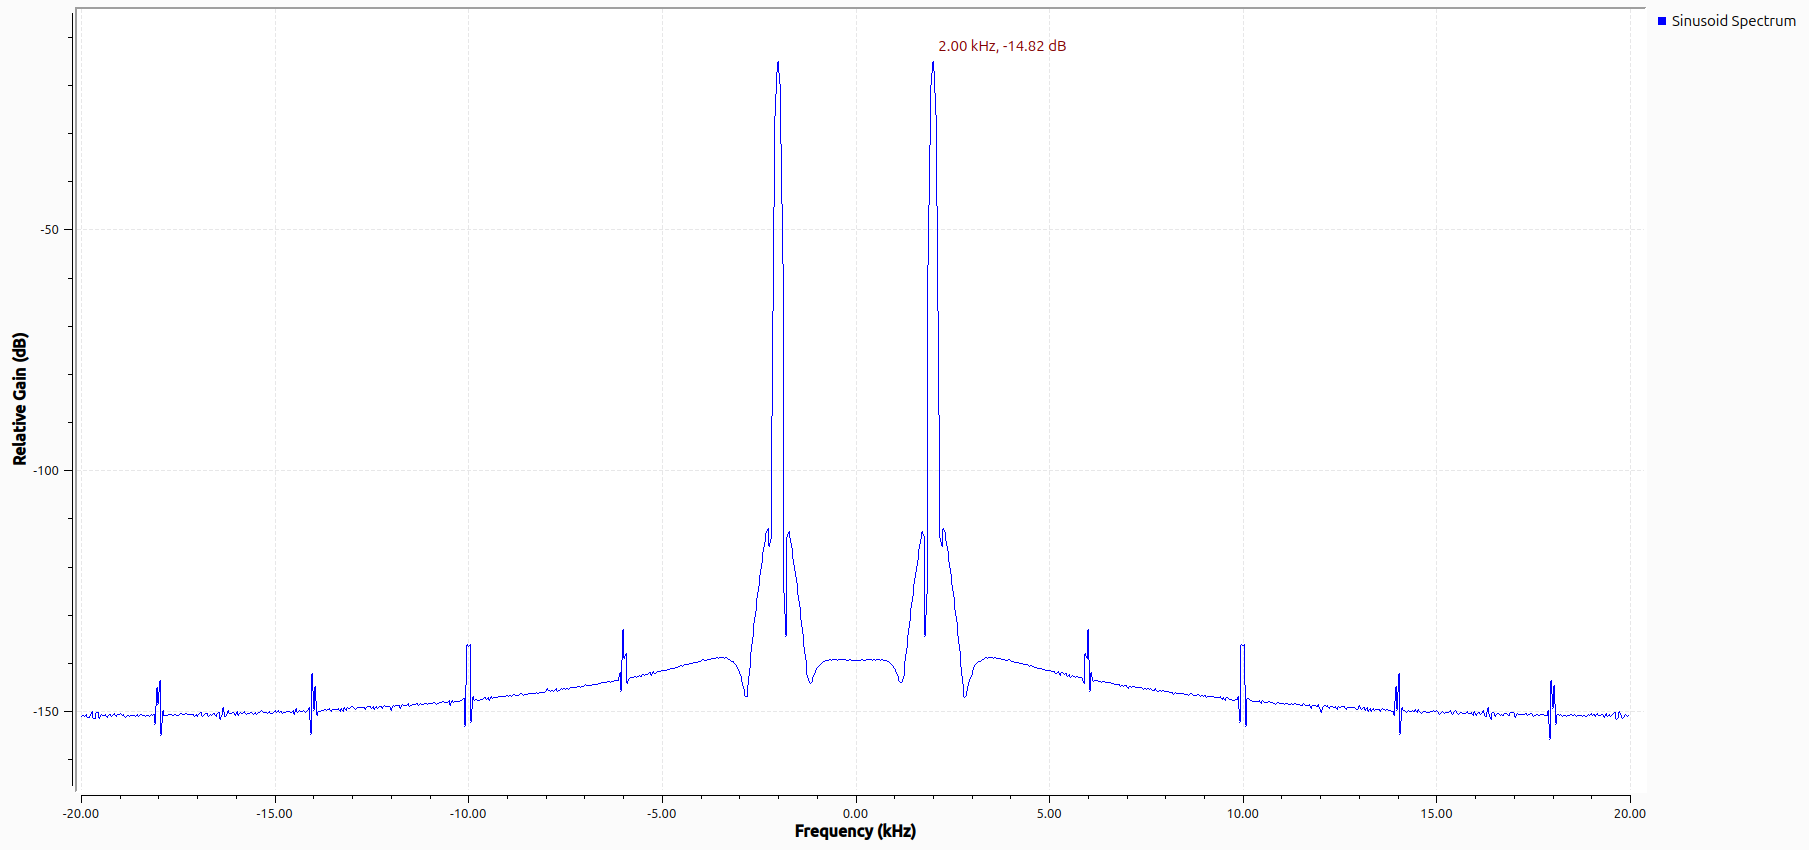
\includegraphics[width=0.7\textwidth]{sampling_rates_freq_domain_40k_samp_rate.png}}}
	\caption{Frequency Response of a Sinusoid Sampled at 40 kHz}
	\label{fig::sampling_rates_freq_domain_40k_samp_rate}
\end{figure}

After increasing the sample rate to 40 kHz, the scope capture looks much more sinusoid-like. This is because there are more samples per period of the sinusoid, which results in less interpolation between samples. The updated scope capture is shown in Figure \ref{fig::sampling_rates_time_domain_40k_samp_rate}.

\begin{figure}[H]
	\centerline{\fbox{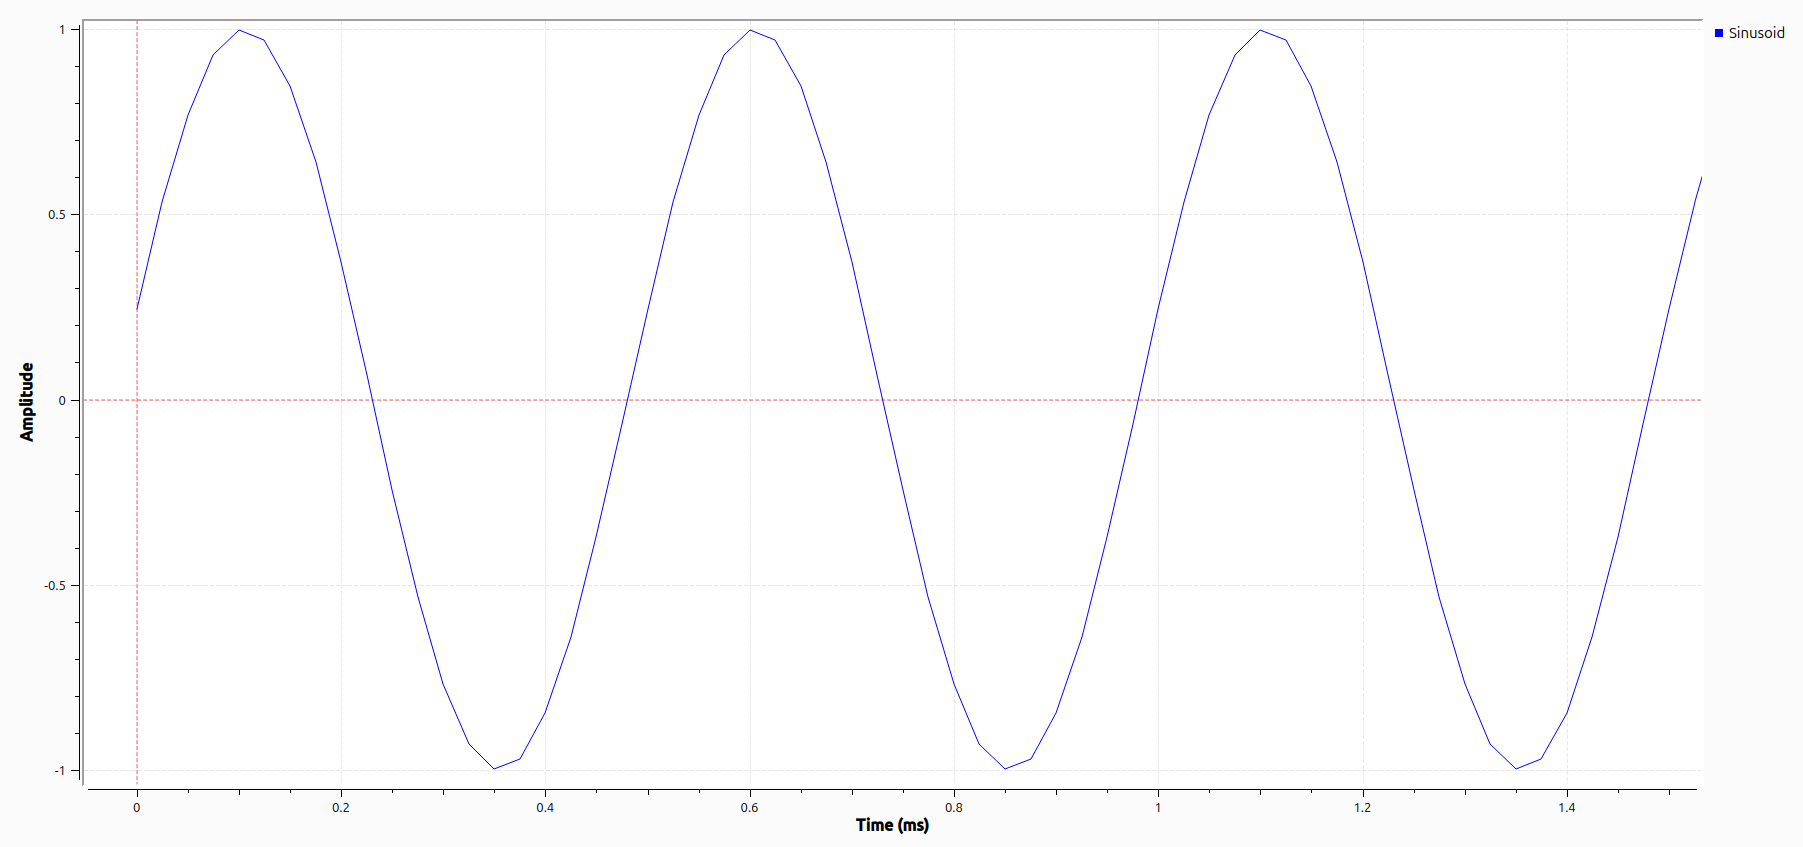
\includegraphics[width=0.7\textwidth]{sampling_rates_time_domain_40k_samp_rate.png}}}
	\caption{Time-Domain Capture of Sinusoid Sampled at 40 kHz}
	\label{fig::sampling_rates_time_domain_40k_samp_rate}
\end{figure}

Now, we adjust the sample rate to 3.5 kHz and measure the peak of the frequency response. We see that it peaks at $\pm$ 1.5 kHz instead of $\pm$ 2 kHz. This is illustrated in Figure \ref{fig::sampling_rates_freq_domain_3_5k_samp_rate}.

\begin{figure}[H]
	\centerline{\fbox{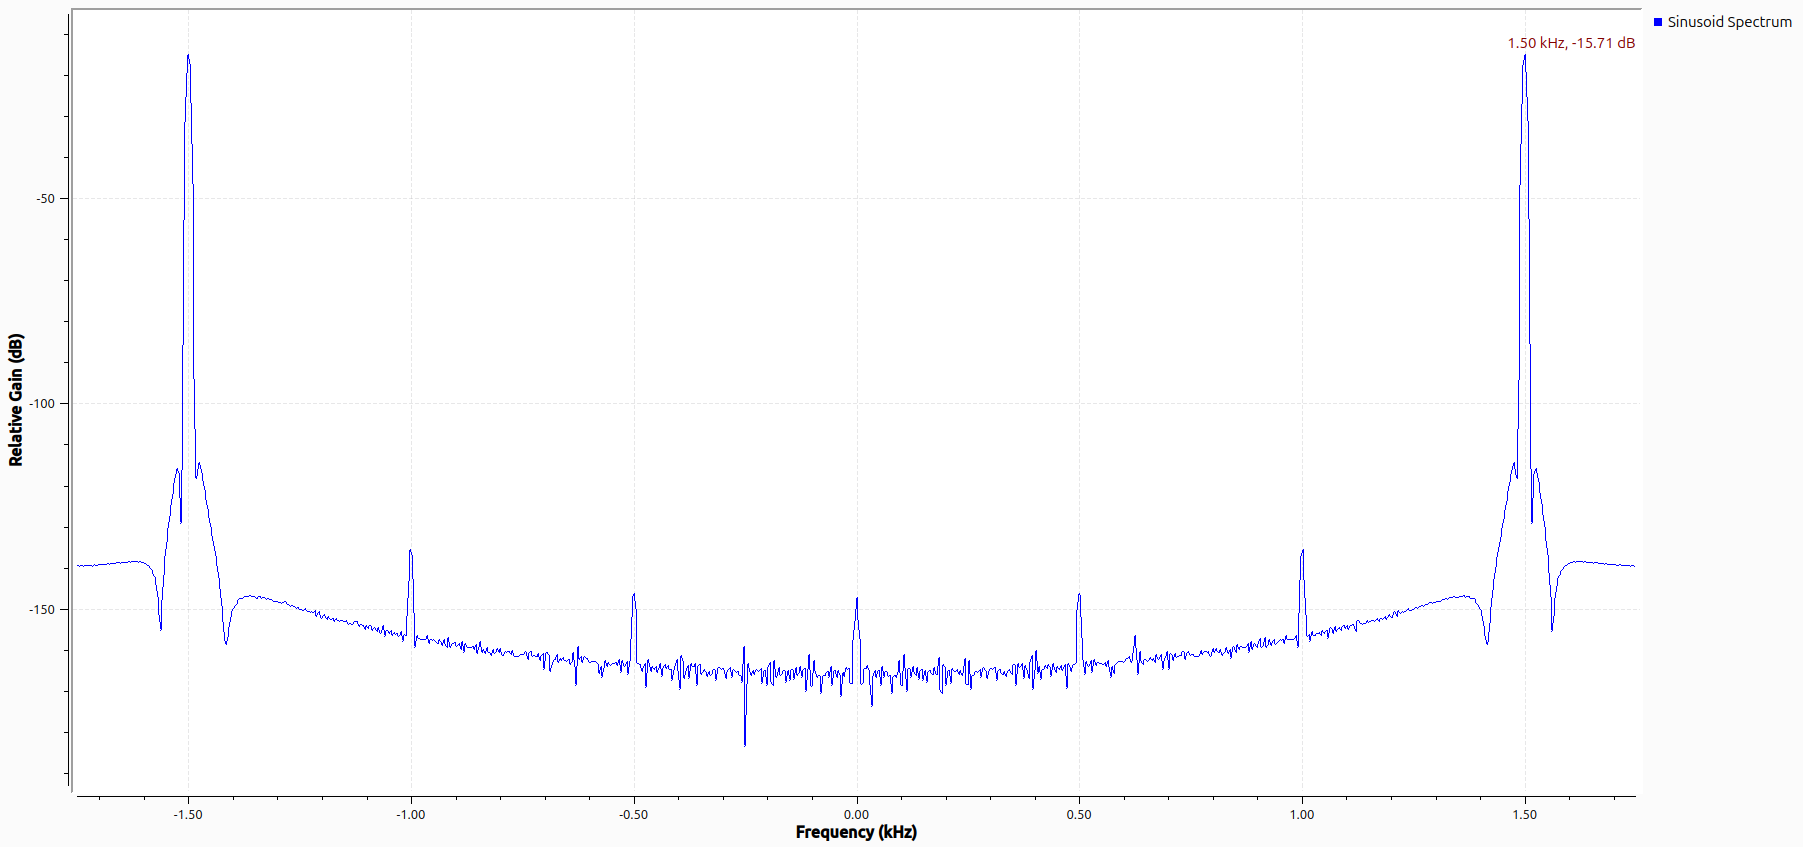
\includegraphics[width=0.7\textwidth]{sampling_rates_freq_domain_3_5k_samp_rate.png}}}
	\caption{Frequency Response of a Sinusoid Sampled at 3.5 kHz}
	\label{fig::sampling_rates_freq_domain_3_5k_samp_rate}
\end{figure}

The phenomenon we observe is called aliasing. Aliasing occurs because the spectrum of a sampled signal wraps into the interval $[-f_s/2, f_s/2)$. In this experiment, the delta function at positive frequency aliases from 2 kHz to -1.5 kHz and the delta function at negative frequency aliases from -2 kHz to 1.5 kHz. As a result, the measured frequency changes by 0.5 kHz, from 2 kHz to 1.5 kHz.

\subsection{Complex Sampling}

Using the flowchart shown in Figure \ref{fig::complex_sampling_experiment}, we investigate the effects of complex sampling. Figure \ref{fig::complex_sampling_freq_domain_10k_samp_rate} shows the frequency response when complex sampling is used instead of real sampling.

\begin{figure}[H]
	\centerline{\fbox{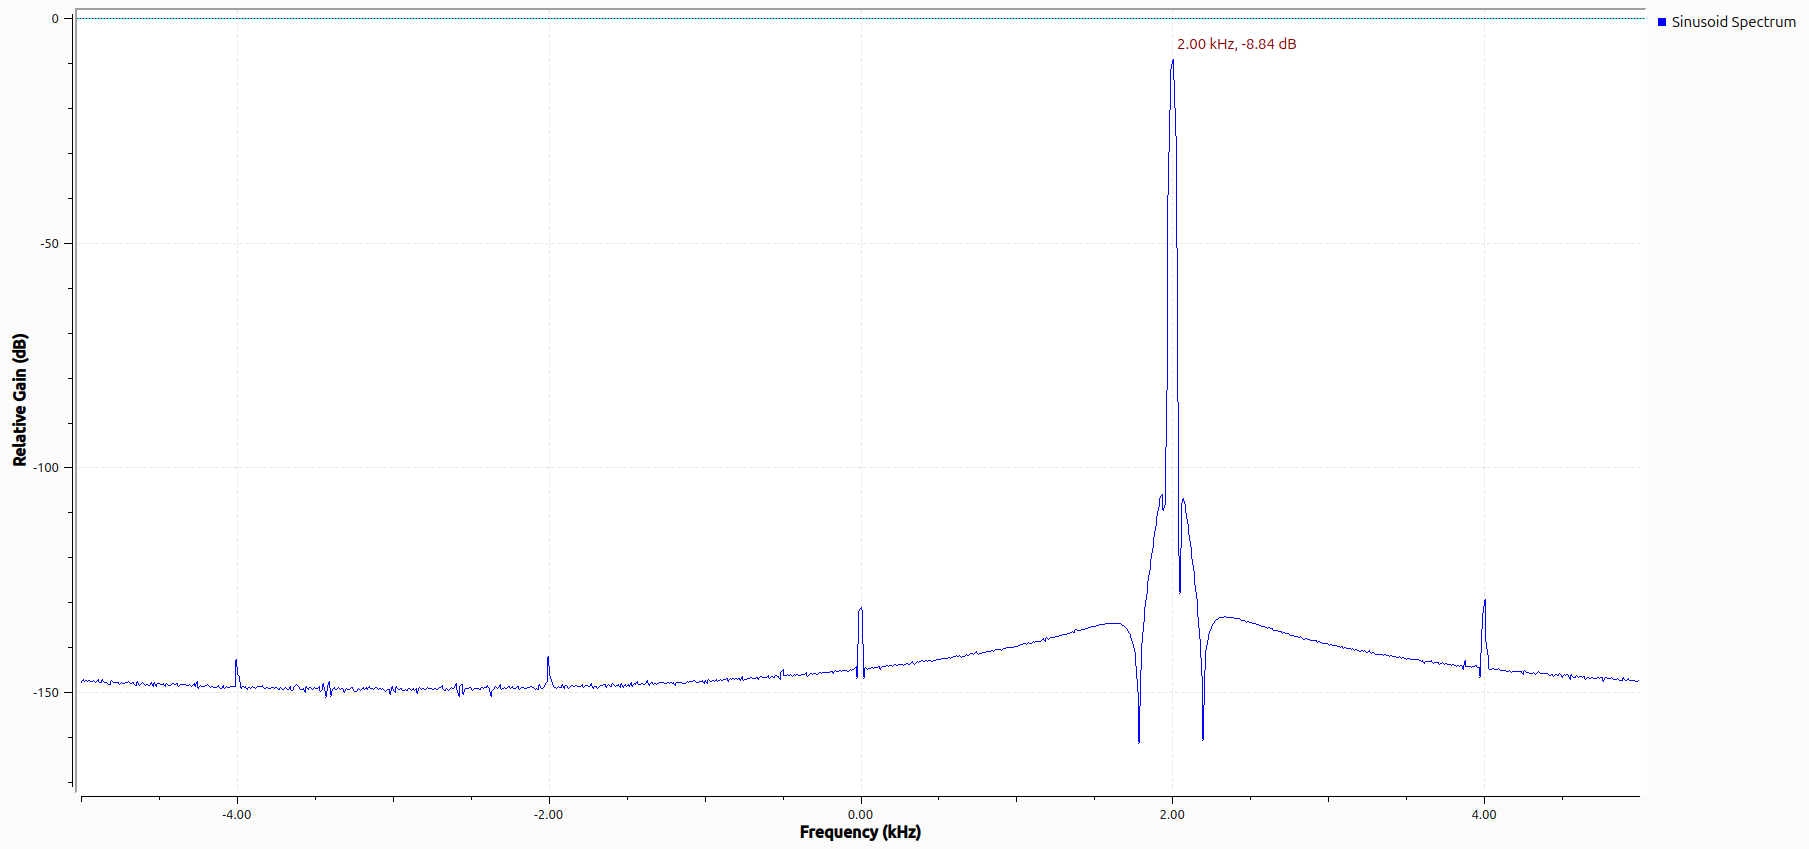
\includegraphics[width=0.7\textwidth]{complex_sampling_freq_domain_10k_samp_rate.png}}}
	\caption{Frequency Response of a Complex Exponential Sampled at 10 kHz}
	\label{fig::complex_sampling_freq_domain_10k_samp_rate}
\end{figure}

Compared to the frequency response shown in Figure \ref{fig::sampling_rates_freq_domain_10k_samp_rate}, the updated frequency response only has a peak at positive frequency. This is expected because the frequency response of a complex exponential is a delta function. Compare this to a sine function, which can be expressed using the inverse Euler formula as:

\begin{equation}
	sin(2{\pi}{f_o}t) = \frac{e^{j2{\pi}{f_o}t} - e^{-j2{\pi}{f_o}t}}{2j}
\end{equation}

It is clear that the sine function can be decomposed into two complex exponentials with positive and negative frequencies resulting in a two-sided spectrum.

When viewed in the time domain, the captured data is composed of 2 channels as illustrated in Figure \ref{fig::complex_sampling_time_domain_10k_samp_rate}. These two channels represent the in-phase (I) and quadrature (Q) components of the signal. They serve as the real and imaginary parts of the complex data stream. The in-phase and quadrature components of the signal are 90 degrees out of phase.

\begin{figure}[H]
	\centerline{\fbox{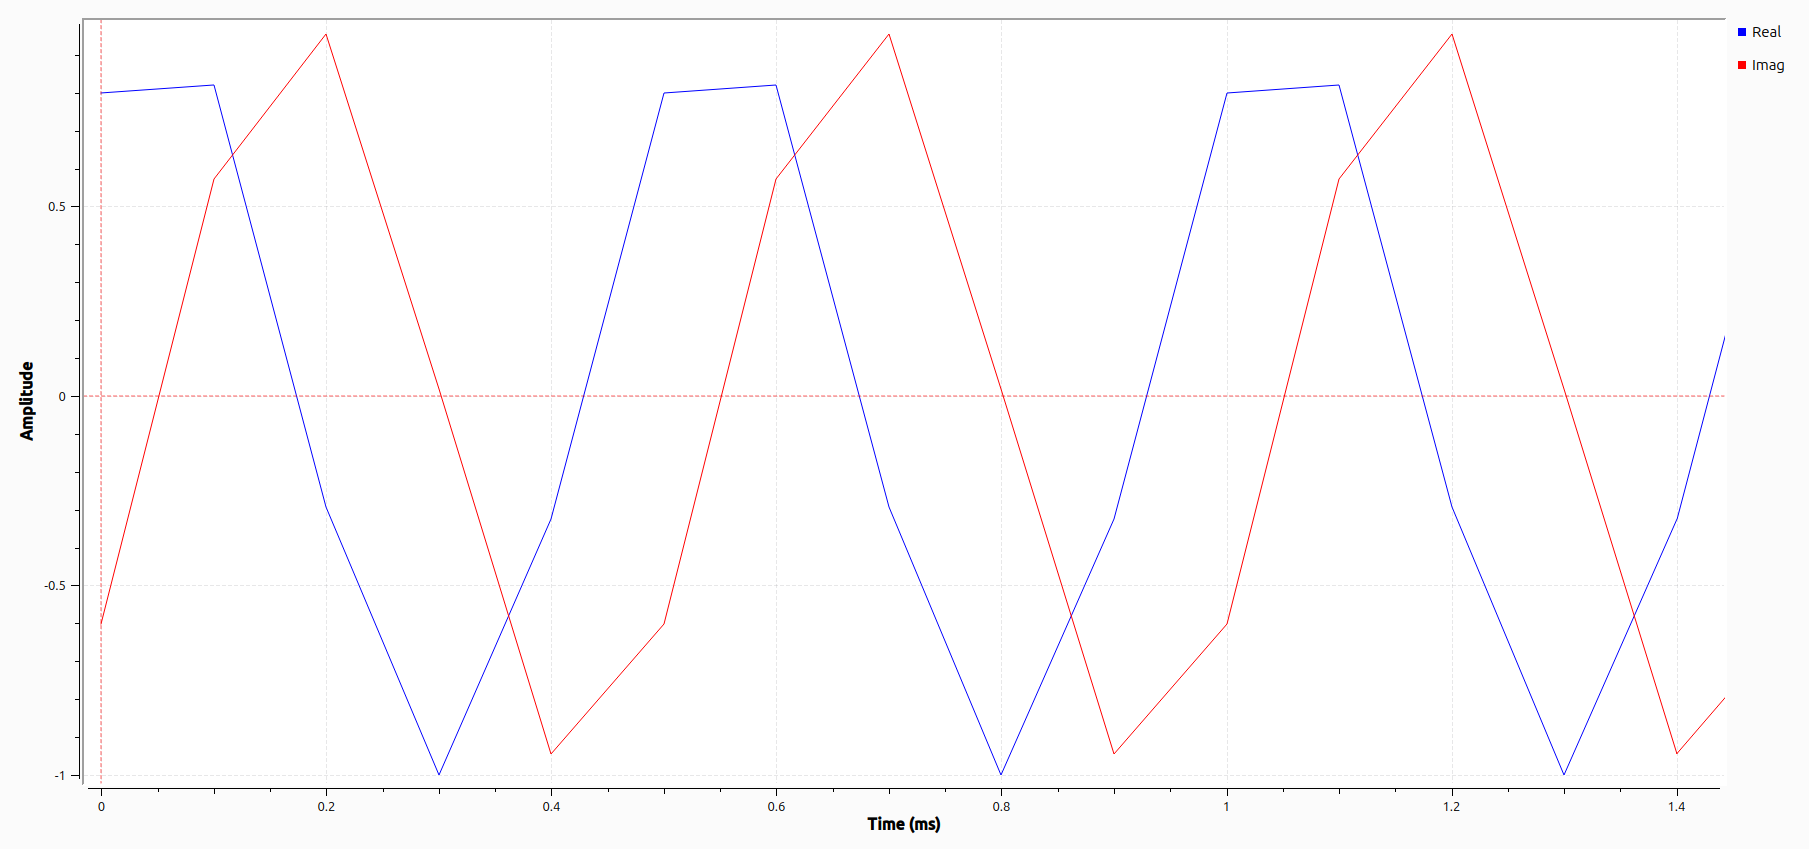
\includegraphics[width=0.7\textwidth]{complex_sampling_time_domain_10k_samp_rate.png}}}
	\caption{Time-Domain Capture of Complex Exponential Sampled at 10 kHz}
	\label{fig::complex_sampling_time_domain_10k_samp_rate}
\end{figure}

After increasing the sample rate to 40 kHz, we see that the amplitude of the real and imaginary parts of the signal are both 1 as expected. This result is captured in Figure \ref{fig::complex_sampling_time_domain_40k_samp_rate}.

\begin{figure}[H]
	\centerline{\fbox{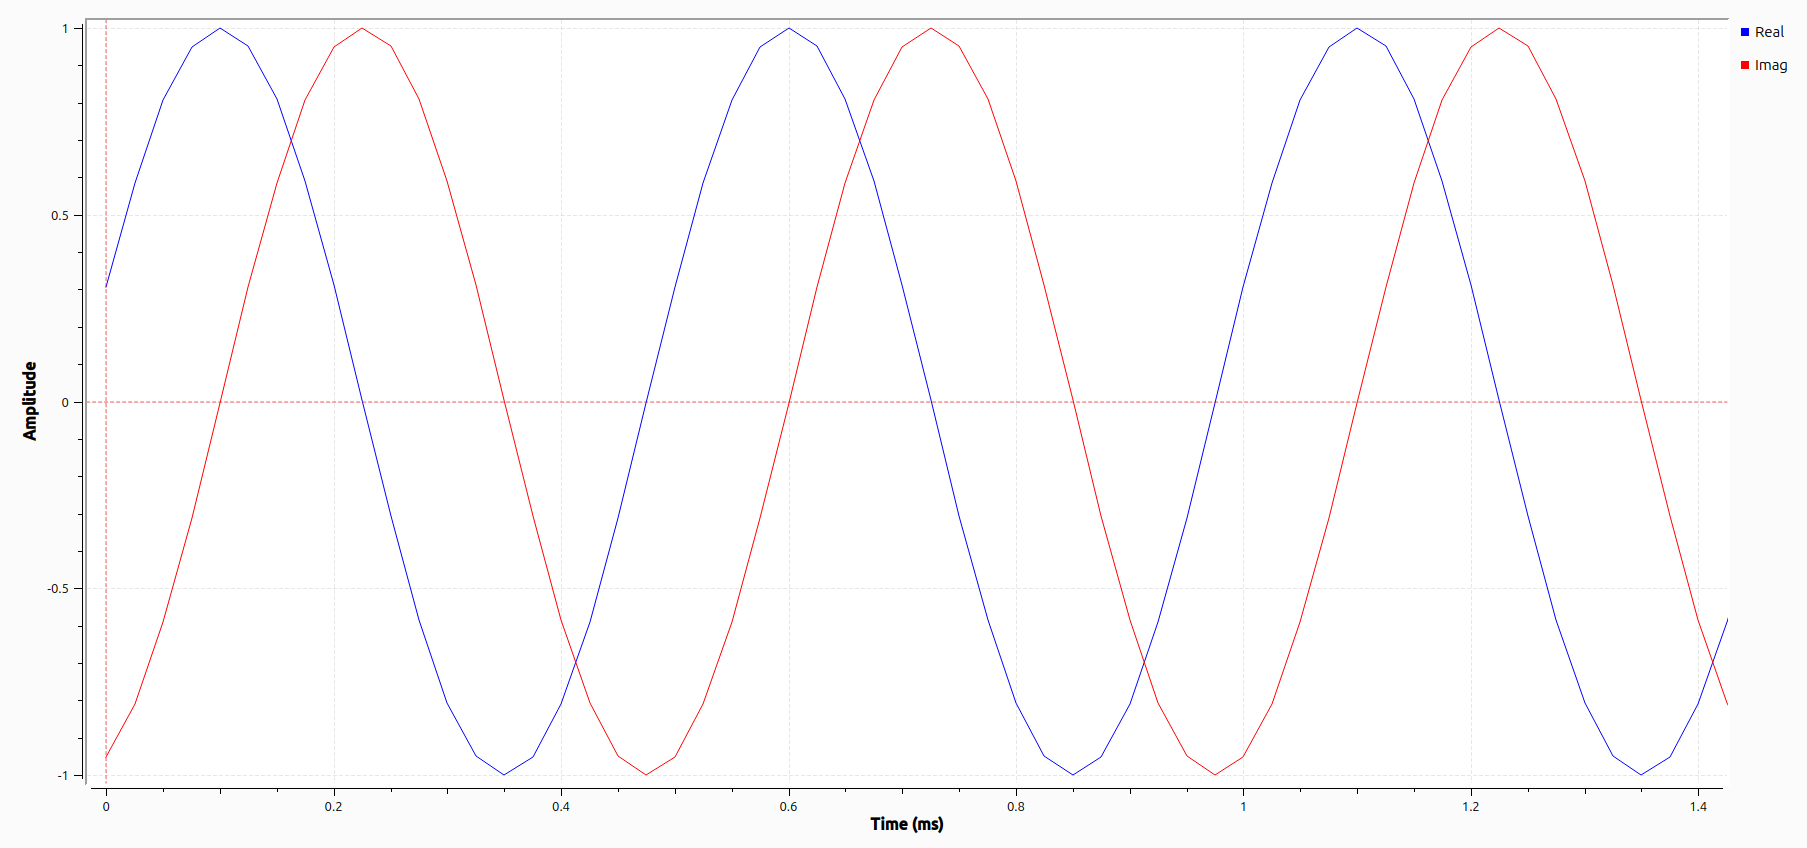
\includegraphics[width=0.7\textwidth]{complex_sampling_time_domain_40k_samp_rate.png}}}
	\caption{Time-Domain Capture of Complex Exponential Sampled at 40 kHz}
	\label{fig::complex_sampling_time_domain_40k_samp_rate}
\end{figure}

We can also measure the peak of the frequency response with the updated sampled rate as illustrated in Figure \ref{fig::complex_sampling_freq_domain_40k_samp_rate}. Doing so, we find a peak of 2 kHz, which is consistent with the data captured at a 10 kHz sampling rate.

\begin{figure}[H]
	\centerline{\fbox{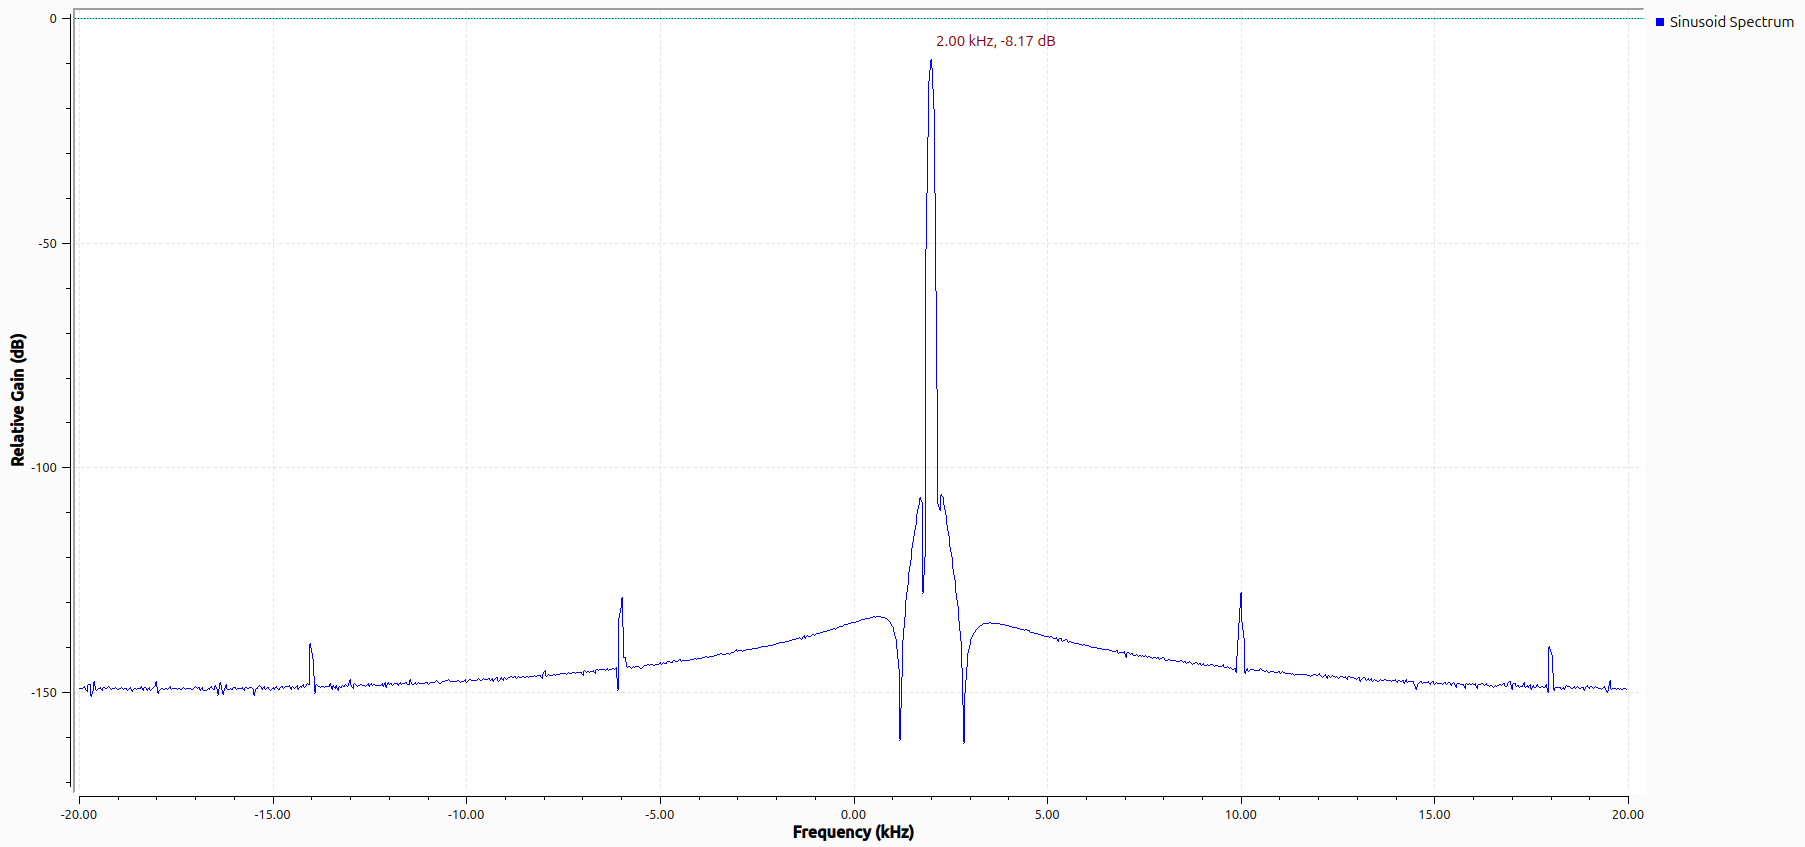
\includegraphics[width=0.7\textwidth]{complex_sampling_freq_domain_40k_samp_rate.png}}}
	\caption{Frequency Response of a Complex Exponential Sampled at 40 kHz}
	\label{fig::complex_sampling_freq_domain_40k_samp_rate}
\end{figure}

Next, we decrease the sampling frequency to the Nyquist rate of 4 kHz (twice the highest frequency) and recollect the frequency response. The updated frequency response is shown in \ref{fig::complex_sampling_freq_domain_4k_samp_rate} and peaks at $\pm 2 kHz$.

\begin{figure}[H]
	\centerline{\fbox{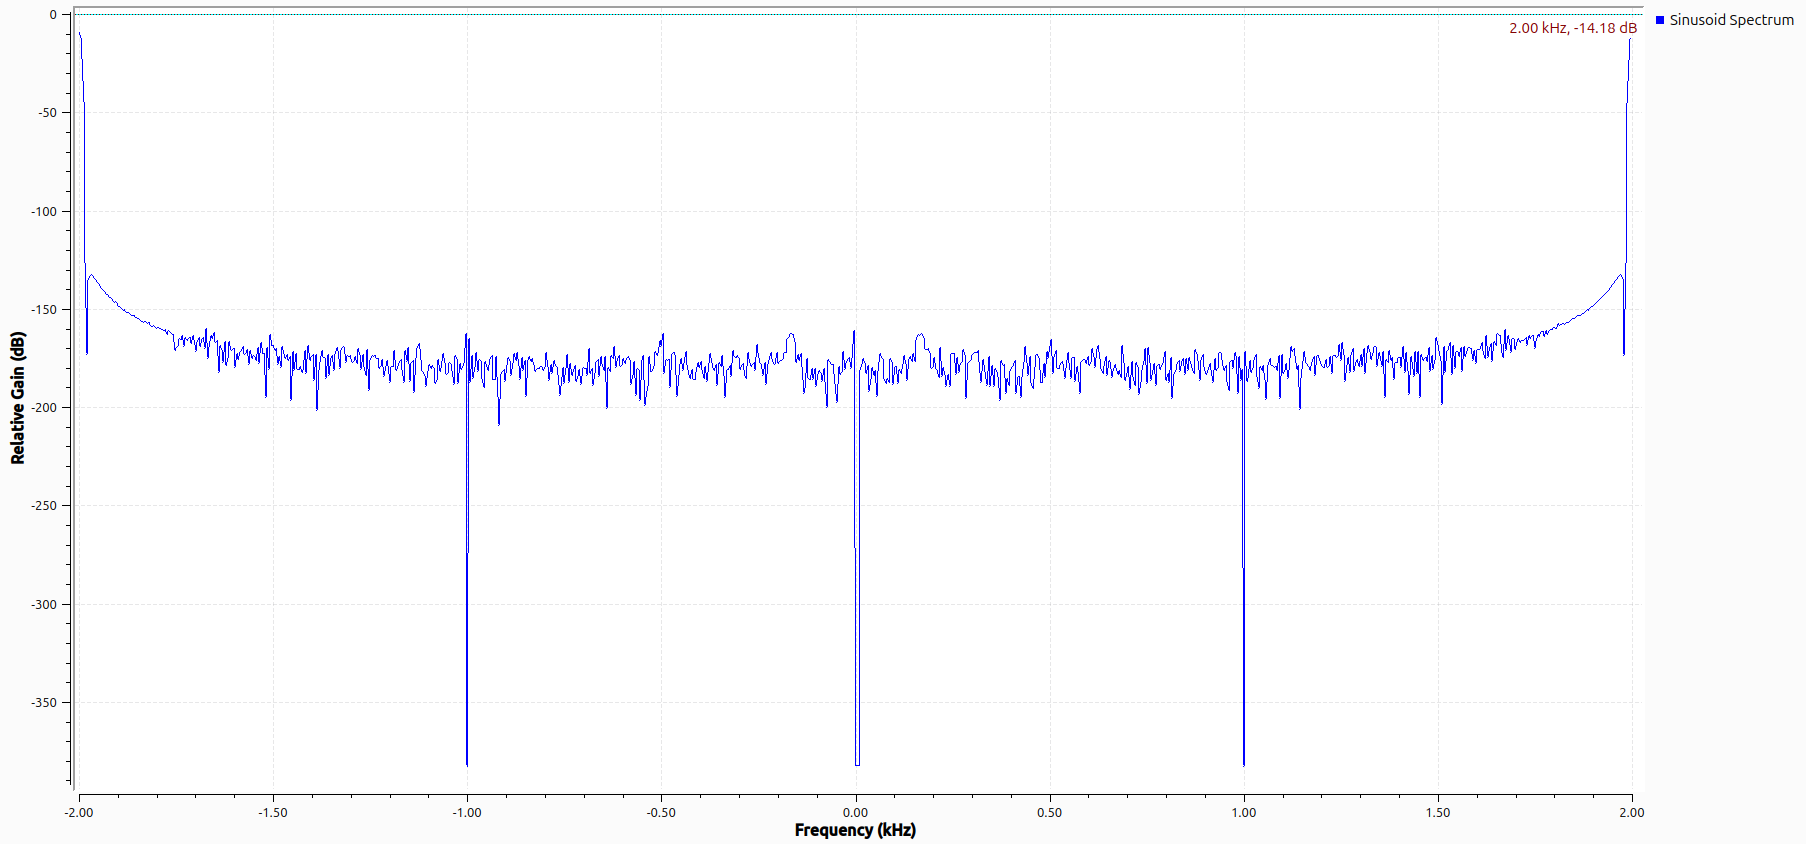
\includegraphics[width=0.7\textwidth]{complex_sampling_freq_domain_4k_samp_rate.png}}}
	\caption{Frequency Response of Complex Exponential Sampled at 4 kHz}
	\label{fig::complex_sampling_freq_domain_4k_samp_rate}
\end{figure}

We expect one delta function in the frequency response, so why do we see two? Well, our frequency response is captured using a windowed subset of samples. Since we only use a subset of samples, our frequency response will not be a delta function but will have a measurable mainlobe and sidelobes. The frequency response will peak at the aliased carrier frequency. Due to the periodicity of the DTFT, what we are seeing is a copy of the mainlobe from different Nyquist zones. One is from the frequency response centered about 0 kHz and the other is from the frequency response centered at -4 kHz. We could also perform an inverse FFT shift on the data and interpret it using frequencies between 0 kHz and 4 kHz. This would make it easier for us to interpret the "two" frequency response peaks as a single peak.

Finally, we continue decreasing the sampling frequency below the Nyquist rate to visualize the effects of aliasing. We display the results at a sampling frequency of 3 kHz. At this sampling rate, the frequency response peaks at -1 kHz as illustrated in Figure \ref{fig::complex_sampling_freq_domain_3k_samp_rate}. At this sampling frequency, the frequency wraps into the interval between $\pm 1.5 kHz$. We can find out the wrapped frequency by adding or subtracting multiples of the sampling frequency. In this case the frequency wraps to 2 kHz - 3 kHz = -1 kHz.

\begin{figure}[H]
	\centerline{\fbox{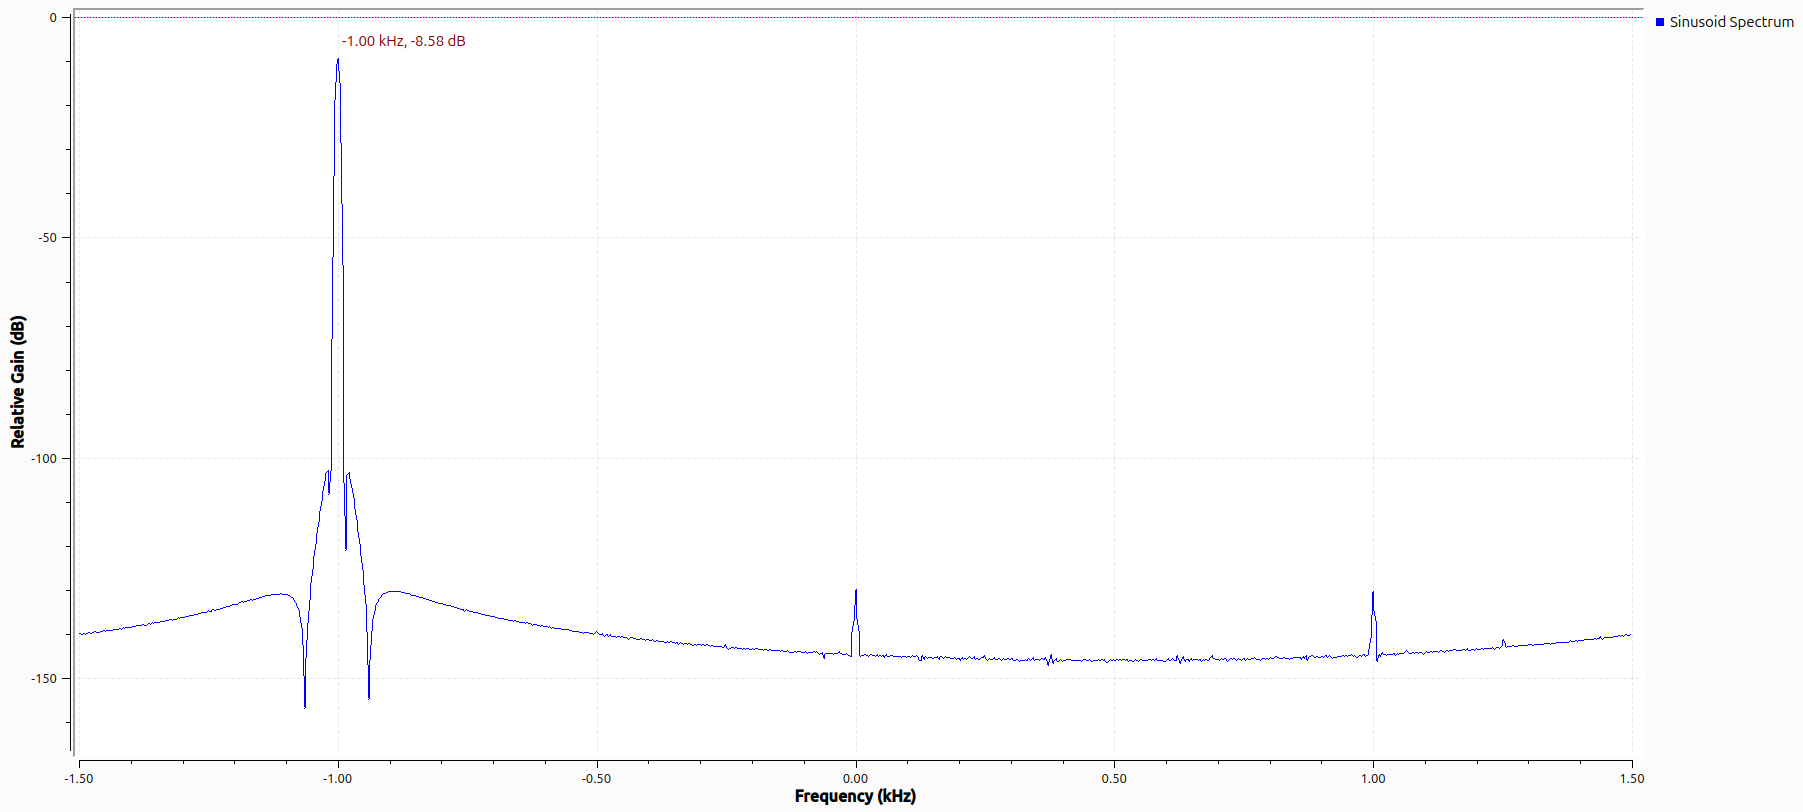
\includegraphics[width=0.7\textwidth]{complex_sampling_freq_domain_3k_samp_rate.png}}}
	\caption{Frequency Response of a Complex Exponential Sampled at 3 kHz}
	\label{fig::complex_sampling_freq_domain_3k_samp_rate}
\end{figure}

\subsection{Frequency Observations}

Using a fixed sample rate, we now vary the frequency of the source and examine what happens for complex and real-sampled data when we exceed the Nyquist frequency.

\subsubsection{Complex-sampled Flowgraph}

For complex-sampled data, we use the flowchart shown in Figure \ref{fig::freq_observations_complex_6k_center_freq} to perform our experiments. The measured frequency increases with increasing frequency and wraps when it cross half the sampling rate (5 kHz), through a phenomenon known as aliasing.

Figure \ref{fig::freq_observations_complex_6k_center_freq} shows the resulting spectrum when the sinusoid center frequency is increased to 6 kHz. Because the sampling frequency is 10 kHz, the frequency will wrap into the interval between $\pm 5 kHz$. We can find out the wrapped (or aliased) frequency by adding or subtracting multiples of the sampling frequency. In this case, the frequency wraps to 6 kHz - 10 kHz = -4 kHz.

\begin{figure}[H]
	\centerline{\fbox{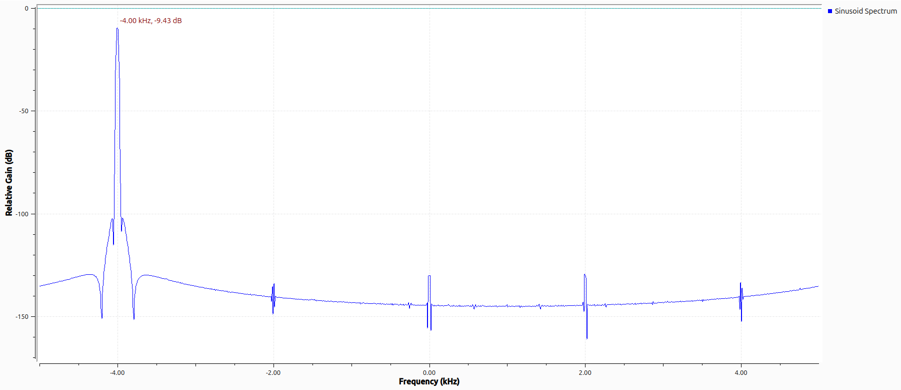
\includegraphics[width=0.7\textwidth]{freq_observations_complex_6k_center_freq.png}}}
	\caption{Frequency Response of a Complex Exponential with 6 kHz Center Frequency}
	\label{fig::freq_observations_complex_6k_center_freq}
\end{figure}

\subsubsection{Real-sampled Flowgraph}

For real-sampled data, we use the flowchart shown in Figure \ref{fig::frequency_observations_real_sampling} to perform our experiments. Compared to the complex-sampled data, the positive and negative sides of the frequency response are symmetric. When increasing the frequency, we see that the frequency appears to increase and then decrease instead of just increase. This is because a sinusoid can be decomposed into two complex exponentials (one with positive and one with negative frequency). The complex exponential with positive frequency center frequency results in an increasing frequency peak, while the complex exponential with negative center frequency results in an decreasing frequency peak.

Figure \ref{fig::freq_observations_real_6k_center_freq} shows the resulting spectrum when the sinusoid center frequency is increased to 6 kHz. Compared to the complex sampled data, the frequency response peaks at $\pm 4 kHz$ instead of just $4 kHz$. Because the sampling frequency is 10 kHz, the frequency will wrap into the interval between $\pm 5 kHz$. We can find out the wrapped (or aliased) frequency by adding or subtracting multiples of the sampling frequency for each peak in the frequency response. In this case, the frequencies wrap to 6 kHz - 10 kHz = -4 kHz and -6 kHz + 10 kHz = 4 kHz. 

\begin{figure}[H]
	\centerline{\fbox{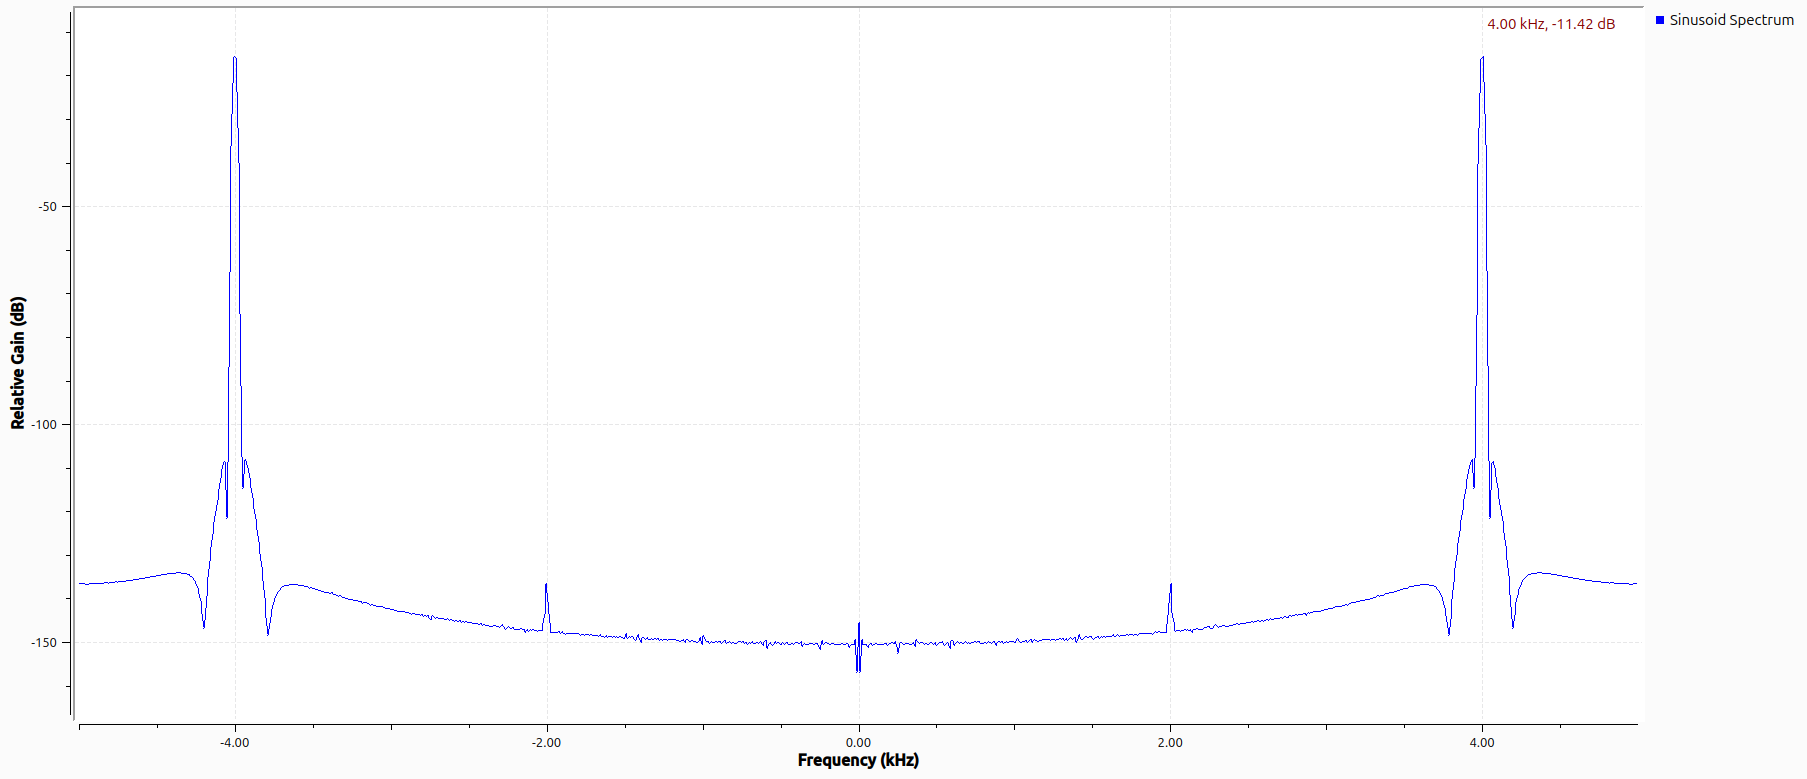
\includegraphics[width=0.7\textwidth]{freq_observations_real_6k_center_freq.png}}}
	\caption{Frequency Response of a Sinusoid with 6 kHz Center Frequency}
	\label{fig::freq_observations_real_6k_center_freq}
\end{figure}

\subsection{I/Q Imbalance}

The effects of I/Q imbalance can be observed using the flowchart shown in Figure \ref{fig::iq_imbalance_experiment}. We start with the default values of 0 magnitude and 0 phase imbalance. Then, we plot the resulting signal in the time and frequency-domain. The results are shown in Figures \ref{fig::iq_imbalance_0_mag_0_phase_time} and \ref{fig::iq_imbalance_0_mag_0_phase_freq} respectively. 

\begin{figure}[H]
	\centerline{\fbox{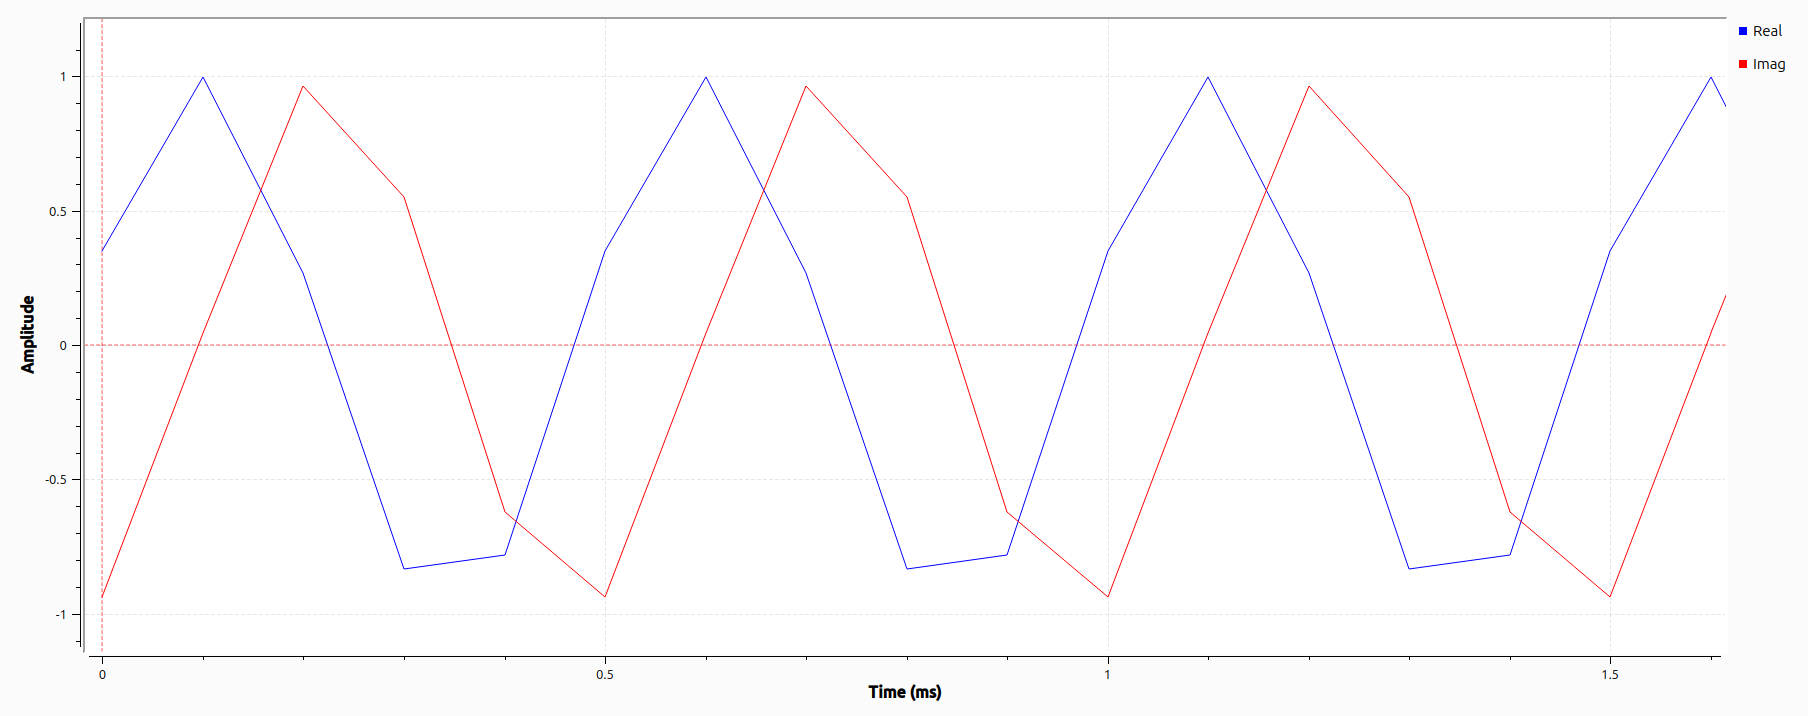
\includegraphics[width=0.7\textwidth]{iq_imbalance_0_mag_0_phase_time.png}}}
	\caption{Time-Domain Capture of Complex Exponential without I/Q Imbalance}
	\label{fig::iq_imbalance_0_mag_0_phase_time}
\end{figure}

\begin{figure}[H]
	\centerline{\fbox{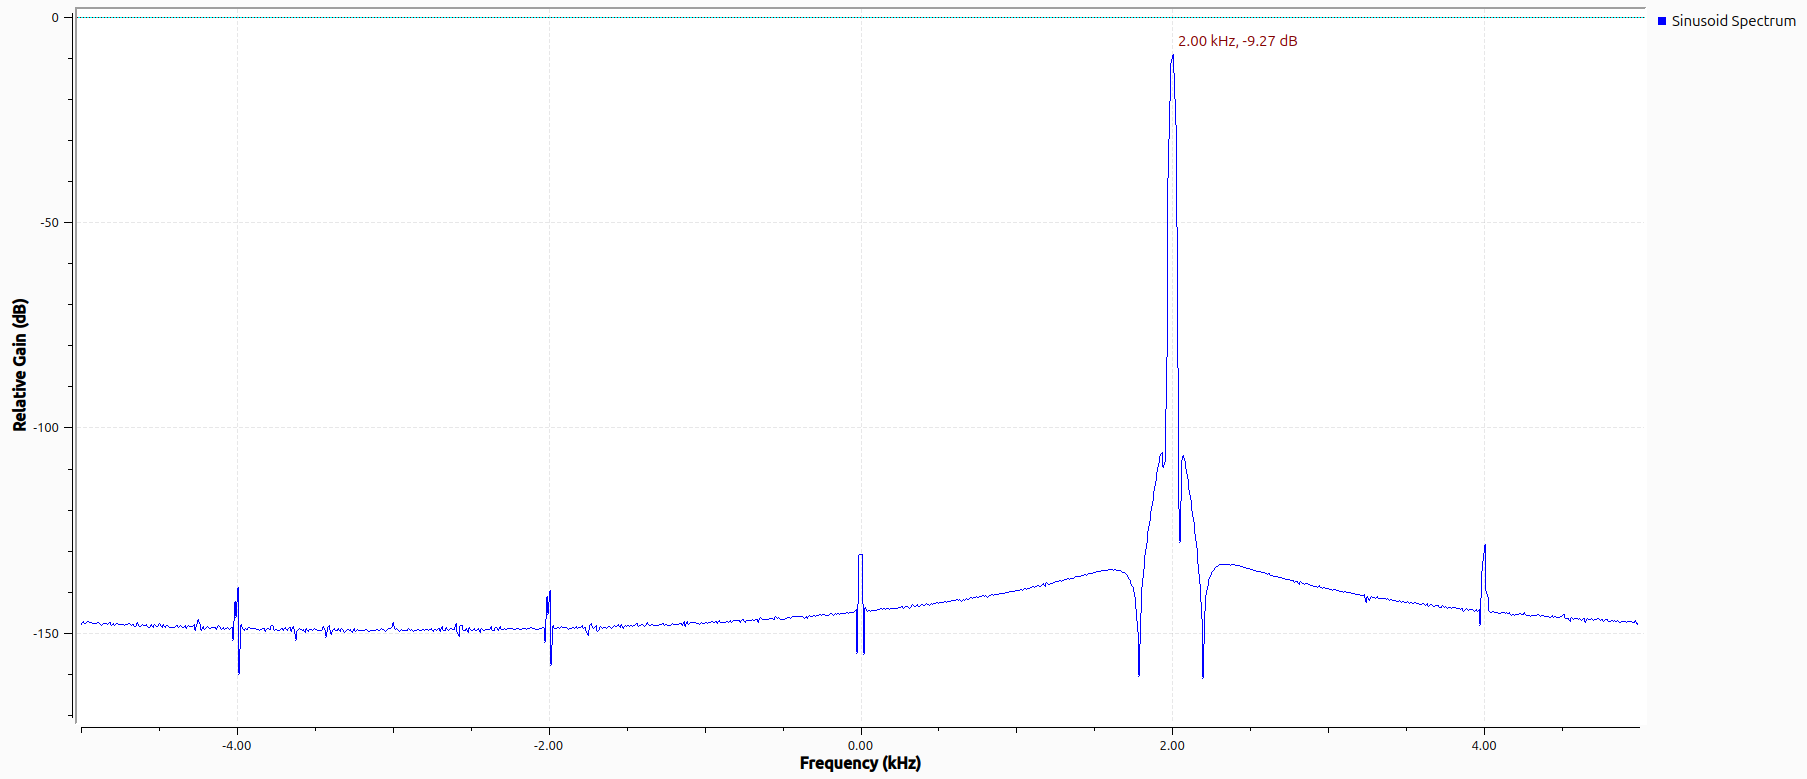
\includegraphics[width=0.7\textwidth]{iq_imbalance_0_mag_0_phase_freq.png}}}
	\caption{Frequency Response of a Complex Exponential without I/Q Imbalance}
	\label{fig::iq_imbalance_0_mag_0_phase_freq}
\end{figure}

As expected, the above plots are identical to those shown in Figures \ref{fig::sampling_rates_time_domain_10k_samp_rate} and  \ref{fig::complex_sampling_freq_domain_10k_samp_rate}.

Next, we investigate the effects of a phase imbalance. As we increase the phase imbalance, we also increase the power of the frequency image. This is illustrated in Figure \ref{fig::iq_imbalance_0_mag_1_phase_freq}, which shows 1 degree of phase imbalance, and Figure \ref{fig::iq_imbalance_0p5_mag_0_phase_freq}, which shows 0.5 dB of amplitude imbalance.

\begin{figure}[H]
	\centerline{\fbox{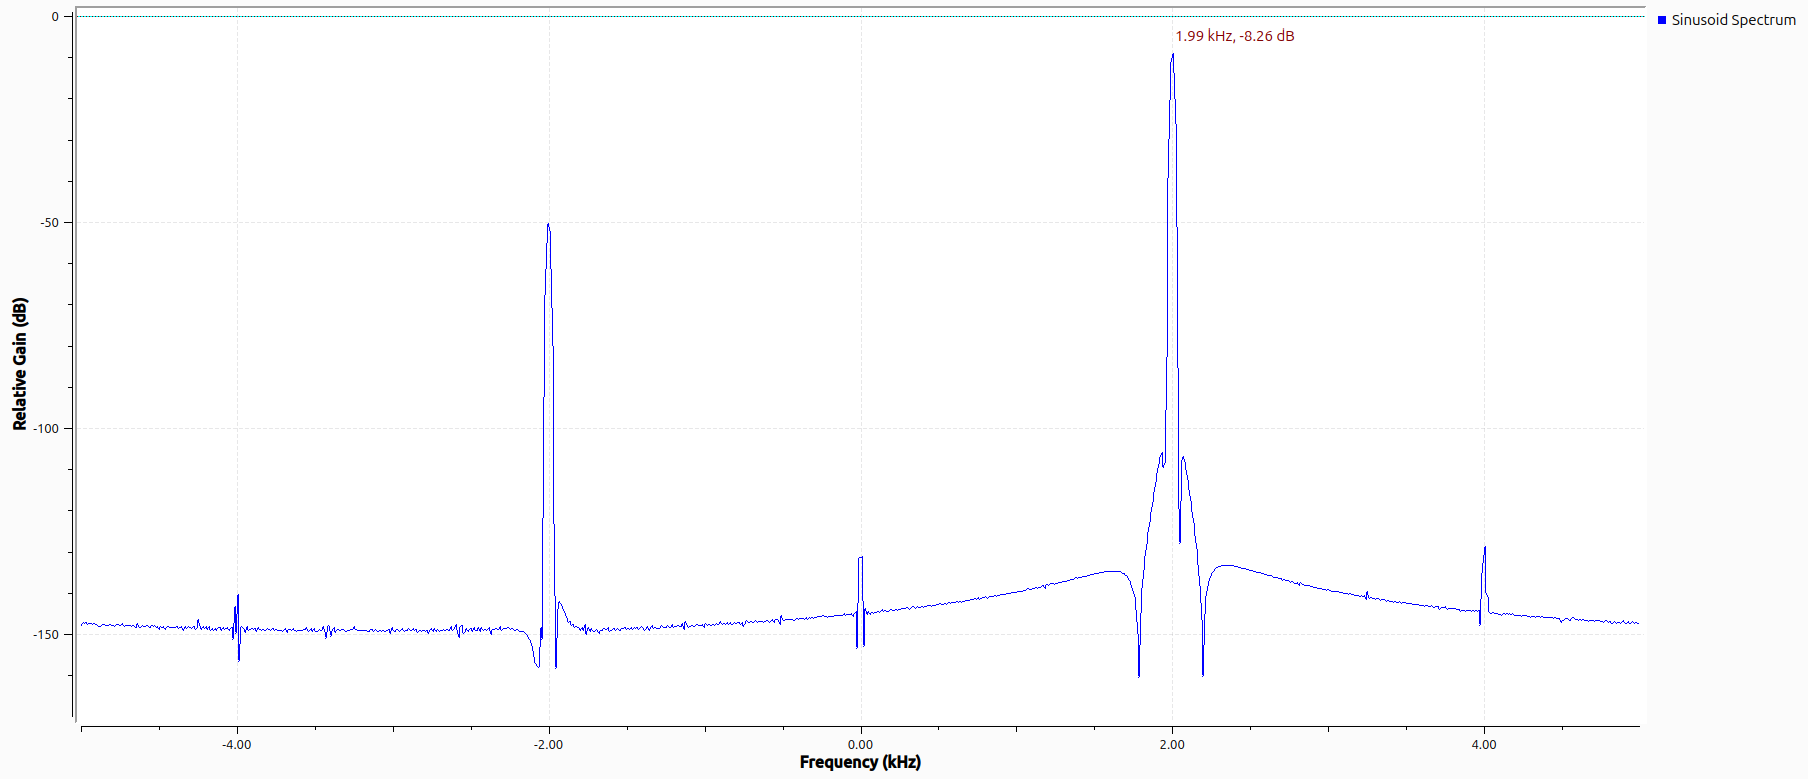
\includegraphics[width=0.7\textwidth]{iq_imbalance_0_mag_1_phase_freq.png}}}
	\caption{Frequency Response of a Complex Exponential with 1 Degree of Phase Imbalance}
	\label{fig::iq_imbalance_0_mag_1_phase_freq}
\end{figure}

\begin{figure}[H]
	\centerline{\fbox{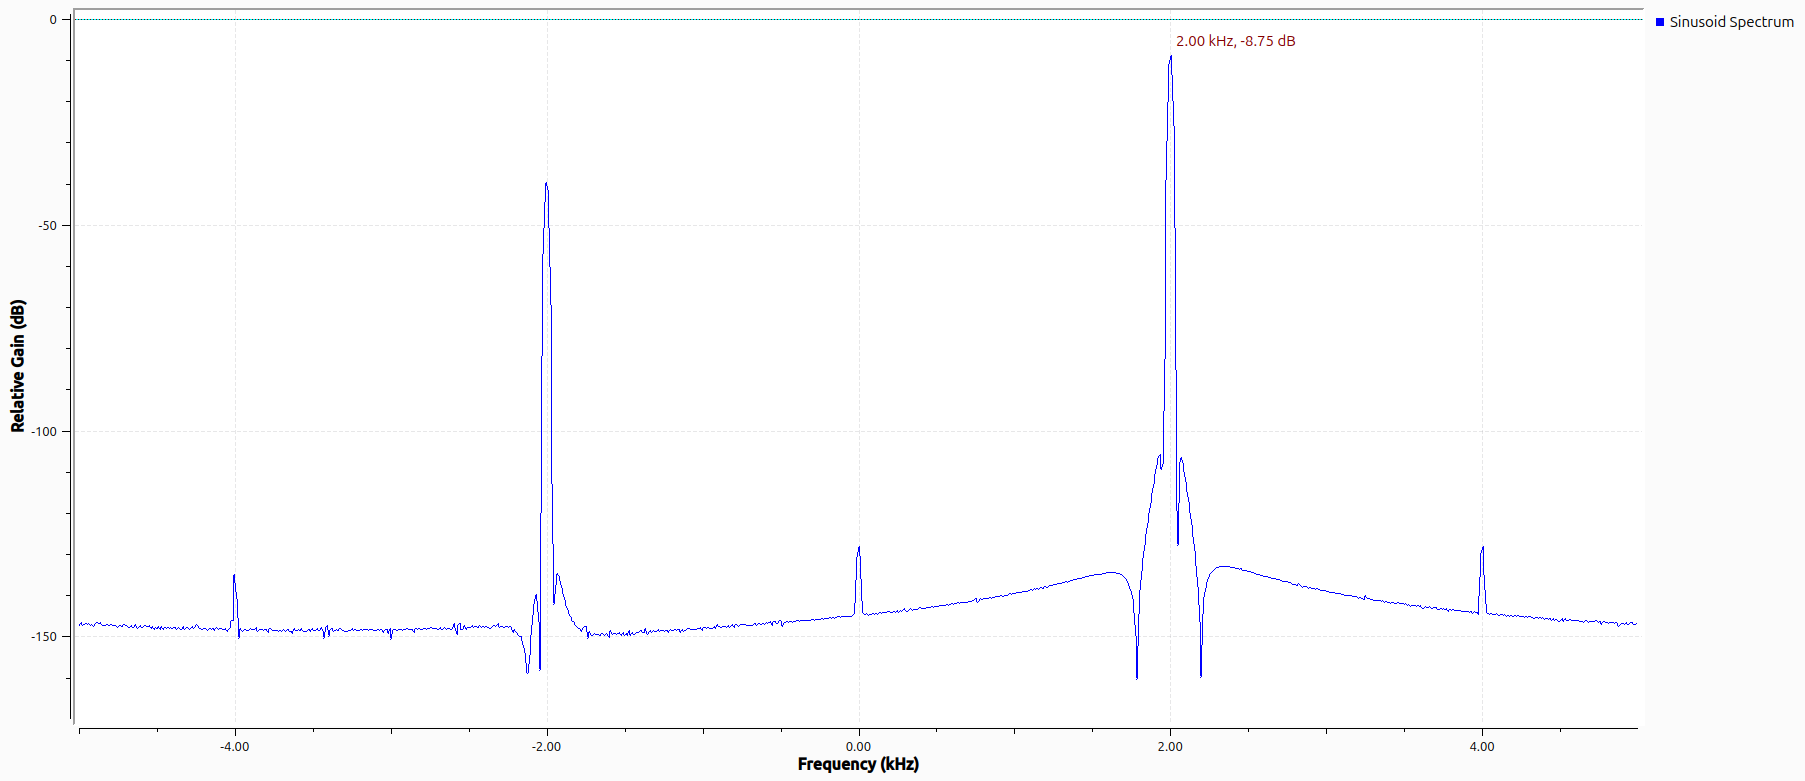
\includegraphics[width=0.7\textwidth]{iq_imbalance_0p5_mag_0_phase_freq.png}}}
	\caption{Frequency Response of a Complex Exponential with 0.5 dB Amplitude Imbalance}
	\label{fig::iq_imbalance_0p5_mag_0_phase_freq}
\end{figure}

The I/Q imbalance block in our flowchart is modeling I/Q imbalance in the transmitter. To understand its effect on the received signal, we must trace the signal from transmitter to receiver. In the transmitter, we are effectively mixing the digitized signal with a complex exponential and then taking the real part of the resulting signal. Here, we also scale the complex exponential by 2 to simplify subsequent equations.

\begin{equation}
	x_{tx}(t) = 2\text{Re}\{x(t)\}\cos(2{\pi}f_ct) - 2\text{Im}\{x(t)\}\sin(2{\pi}f_ct)
\end{equation}

Applying Inverse Euler's formula, we obtain:

\begin{equation}
	x_{tx}(t) = \text{Re}\{x(t)\}(e^{j2{\pi}f_ct} + e^{-j2{\pi}f_ct}) + j\text{Im}\{x(t)\}(e^{j2{\pi}f_ct} - e^{-j2{\pi}f_ct})
\end{equation}

In the receiver, we are effectively mixing the received signal to baseband with another complex exponential and then filtering out the high frequency component. After performing these operations, we obtain the expected result:
 
\begin{equation}
	x_{rx}(t) = \text{Re}\{x(t)\}\ + j\text{Im}\{x(t)\}
\end{equation}

When we apply I/Q imbalance in the transmitter, we obtain the following for the transmitted signal:

\begin{equation}
	x_{tx}(t) = 2(1+\varepsilon)\text{Re}\{x(t)\}\cos(2{\pi}f_ct + \phi) - 2\text{Im}\{x(t)\}\sin(2{\pi}f_ct)
\end{equation}

Applying Inverse Euler's formula, we obtain:

\begin{equation}
	x_{tx}(t) = (1+\varepsilon)\text{Re}\{x(t)\}(e^{j(2{\pi}f_ct+\phi)} + e^{-j(2{\pi}f_ct+\phi)}) + j\text{Im}\{x(t)\}(e^{j2{\pi}f_ct} - e^{-j2{\pi}f_ct})
\end{equation}

The received signal with I/Q imbalance is then given as follows:

\begin{equation}
	x_{rx}(t) = (1+\varepsilon)e^{j\phi}\text{Re}\{x(t)\} + j\text{Im}\{x(t)\}
\end{equation}

Substituting, a complex exponential for the signal $x(t)$ we obtain the following:
\begin{align}
	x_{rx}(t) &= (1+\varepsilon)e^{j\phi}\cos(2{\pi}f_0t) + j\sin(2{\pi}f_0t) \\
	&= 0.5(1+\varepsilon)e^{j\phi}(e^{j2{\pi}f_0t} + e^{-j2{\pi}f_0t}) + 0.5(e^{j2{\pi}f_0t} - e^{-j2{\pi}f_0t})\\
	&= 0.5[(1+\varepsilon)e^{j\phi} + 1]e^{j2{\pi}f_0t} + 0.5[(1+\varepsilon)e^{j\phi} - 1]e^{-j2{\pi}f_0t} \label{eq::rx_signal_iq_imbalance}
\end{align}

The power ratio between the frequency response at $f_0$ and $-f_0$ is given by: 
\begin{equation}
	P_r = \frac{(1-(1+\varepsilon)\cos\phi)^2 + (1+\varepsilon)^2\sin^2\phi}{(1+(1+\varepsilon)\cos\phi)^2 + (1+\varepsilon)^2\sin^2\phi} = \frac{1-2(1+\varepsilon)\cos\phi+(1+\varepsilon)^2}{1+2(1+\varepsilon)\cos\phi+(1+\varepsilon)^2}
\end{equation}

For phase imbalance only, this reduces to:

\begin{equation}
	P_r = \frac{1-\cos\phi}{1+\cos\phi} \label{eq::image_power_ratio_phase_imbalance}
\end{equation}

Similarly, for amplitude imbalance, this reduces to:

\begin{equation}
	P_r = \frac{1-2(1+\varepsilon)+(1+\varepsilon)^2}{1+2(1+\varepsilon)+(1+\varepsilon)^2} = \frac{(1-(1+\varepsilon))^2}{(1+(1+\varepsilon))^2} = \frac{\varepsilon^2}{(2+\varepsilon)^2} \label{eq::image_power_ratio_amplitude_imbalance}
\end{equation}

The image power ratio observed in Figure \ref{fig::iq_imbalance_0_mag_1_phase_freq} is consistent with Equation \ref{eq::image_power_ratio_phase_imbalance}. The equation explains why the image power increases with increasing phase imbalance for $0^{\circ} \leq \phi \leq 180^{\circ}$. Similarly, the image power ratio observed in Figure \ref{fig::iq_imbalance_0p5_mag_0_phase_freq} is consistent with Equation \ref{eq::image_power_ratio_amplitude_imbalance}. The equation explains why the image power increases with increasing amplitude imbalance for $\varepsilon \geq 0$.

Next, we observe the constellation sink output. The constellation sink displays a scatter plot of the samples on the I/Q plane. For the default sample rate of 10 kHz, we observe 5 evenly spaced samples captured each period of the complex exponential. The resulting constellation is shown in Figure \ref{fig::iq_imbalance_0_mag_0_phase_10k_samp_rate_const}.
 
\begin{figure}[H]
	\centerline{\fbox{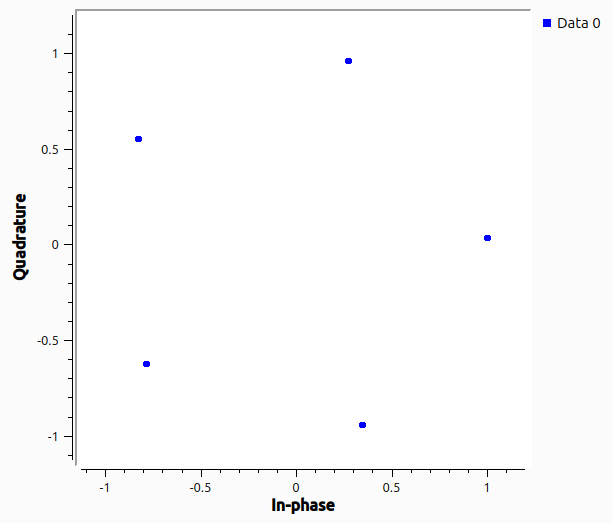
\includegraphics[width=0.4\textwidth]{iq_imbalance_0_mag_0_phase_10k_samp_rate_const.png}}}
	\caption{Constellation with 10 kHz Sample Rate}
	\label{fig::iq_imbalance_0_mag_0_phase_10k_samp_rate_const}
\end{figure}

In general, we will see $N$ unique samples in the constellation, where $N$ is the period of the sampled signal. $N$ must be an integer. As a result, $N$ is not always the sampling rate ($f_s$) divided by the center frequency ($f_o$). $N$ is instead defined as follows:

\begin{equation}
	\frac{f_o}{f_s} = \frac{M}{N} \label{eq::period_of_discrete_signal}
\end{equation}

where $N, M \in \mathcal{Z}$. Here $N=f_s/\text{gcd}(f_o,f_s)$ is the period of the sampled signal, and $M=f_o/\text{gcd}(f_o,f_s)$ is the number of input signal cycles in a period of the sampled signal. When we use a sampling rate of 39.8 kHz, we find that $M=10$ and $N=199$. Thus, we will see 199 unique samples in the constellation. The constellation with a sampling rate of 39.8kHz is shown in Figure \ref{fig::iq_imbalance_0_mag_0_phase_39p8k_samp_rate_const}.

\begin{figure}[H]
	\centerline{\fbox{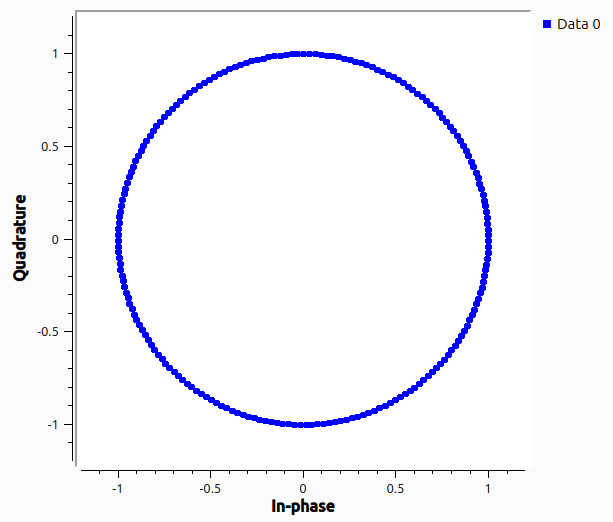
\includegraphics[width=0.4\textwidth]{iq_imbalance_0_mag_0_phase_39p8k_samp_rate_const.png}}}
	\caption{Constellation with 39.8 kHz Sample Rate}
	\label{fig::iq_imbalance_0_mag_0_phase_39p8k_samp_rate_const}
\end{figure}

For sampling rates that are multiples of the center frequency, we will see more points in the constellation as we increase the sampling rate. However, in general, we must use Equation \ref{eq::period_of_discrete_signal} to determine the number of points in the constellation. With the updated sampling rate, we see that the captured samples trace a unit circle in the I/Q plane.

Next, we capture the constellation with I/Q imbalance. However, we continue using a sampling rate of 39.8 kHz when performing this subsequent capture. Note that this deviates slightly from what was requested, but it helps us to better visualize the effects of I/Q imbalance. Figure \ref{fig::iq_imbalance_0_mag_6_phase_39p8k_samp_rate_const} shows the resulting constellation with 6 degrees of I/Q phase imbalance, and Figure \ref{fig::iq_imbalance_1_mag_0_phase_39p8k_samp_rate_const} shows the resulting constellation with 1 dB of I/Q amplitude imbalance.

\begin{figure}[H]
	\centerline{\fbox{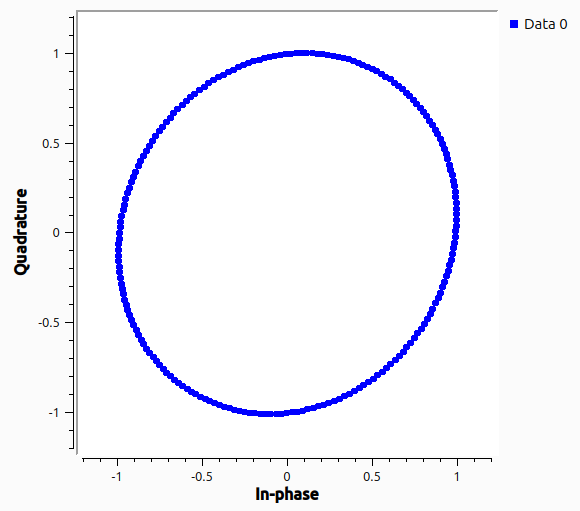
\includegraphics[width=0.4\textwidth]{iq_imbalance_0_mag_6_phase_39p8k_samp_rate_const.png}}}
	\caption{Constellation with 39.8 kHz Sample Rate and 6 Degrees of I/Q Phase Imbalance}
	\label{fig::iq_imbalance_0_mag_6_phase_39p8k_samp_rate_const}
\end{figure}

\begin{figure}[H]
	\centerline{\fbox{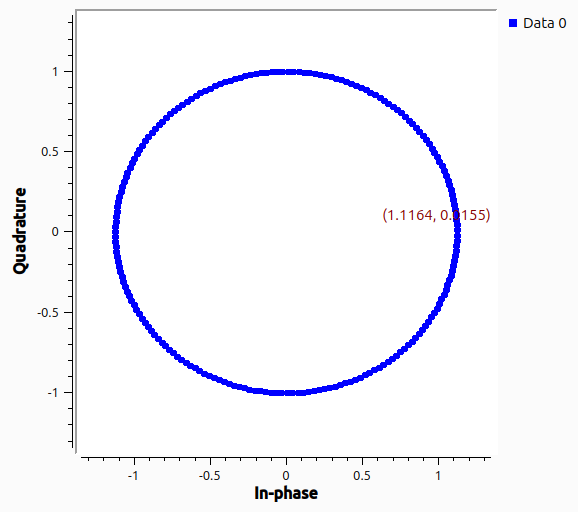
\includegraphics[width=0.4\textwidth]{iq_imbalance_1_mag_0_phase_39p8k_samp_rate_const.png}}}
	\caption{Constellation with 39.8 kHz Sample Rate and 1 dB of I/Q Amplitude Imbalance}
	\label{fig::iq_imbalance_1_mag_0_phase_39p8k_samp_rate_const}
\end{figure}

To better understand what the effects of I/Q imbalance on the constellations, we can rewrite Equation \ref{eq::rx_signal_iq_imbalance} in the following form:
\begin{align}
	x_{rx}(t) &= (1+\varepsilon)(\cos\phi + j\sin\phi)\cos(2{\pi}f_0t) + j\sin(2{\pi}f_0t) \\[6 pt]
	&= (1+\varepsilon)\cos\phi\cos(2{\pi}f_0t) + j((1+\varepsilon)\sin\phi\cos(2{\pi}f_0t) + \sin(2{\pi}f_0t)) \\[6 pt]
	&= (1+\varepsilon)\cos\phi\cos(2{\pi}f_0t) + j((1+\varepsilon)\sin\phi\sin(2{\pi}f_0t + \pi/2) + \sin(2{\pi}f_0t)) \\
	&= (1+\varepsilon)\cos\phi\cos(2{\pi}f_0t) + j\sqrt{1+(1+\varepsilon)^2\sin^2\phi}\sin(2{\pi}f_0t + \text{atan}((1+\varepsilon)\sin\phi)) \label{eq::iq_imbalance_revisited}
\end{align}

For phase imbalance only, Equation \ref{eq::iq_imbalance_revisited} reduces as follows:

\begin{equation}
	x_{rx}(t) = \cos\phi\cos(2{\pi}f_0t) + j\sqrt{1+\sin^2\phi}\sin(2{\pi}f_0t + \text{atan}(\sin\phi)) \label{eq::received_signal_phase_imbalance}
\end{equation}

Similarly, for amplitude imbalance only, Equation \ref{eq::iq_imbalance_revisited} reduces as follows:

\begin{equation}
	x_{rx}(t) = (1+\epsilon)\cos(2{\pi}f_0t) + j\sin(2{\pi}f_0t)
\label{eq::received_signal_amplitude_imbalance}
\end{equation}

The results of Figure \ref{fig::iq_imbalance_0_mag_6_phase_39p8k_samp_rate_const} can be explained using Equation \ref{eq::received_signal_phase_imbalance}. For increasing amounts of phase imbalance, the constellation becomes a diagonally-oriented ellipsoid. This is because the imaginary part of the data peaks at a phase of $90^{\circ} - \text{atan}(\sin\phi)$ instead of a phase of $90^{\circ}$, while the real part of the data peaks at a phase of $0^{\circ}$. The peak of the imaginary part of the data also increases with increasing phase imbalance, while the peak of the real part of the data decreases with increasing phase imbalance. Similarly, the results of Figure \ref{fig::iq_imbalance_1_mag_0_phase_39p8k_samp_rate_const} can be explained using Equation \ref{eq::received_signal_amplitude_imbalance}. For increasing amounts of amplitude imbalance, we see the constellation stretch along the real-axis to $1+\varepsilon$, while the constellation does not stretch along the imaginary axis.

\subsection{Adding Noise}

This experimented highlights the impact of additive noise on time-domain data, frequency-domain data, and resulting constellations. Figure \ref{fig::noise_time_domain_10dB_snr} shows time-domain data with additive white Gaussian noise (AWGN) that results in a 10 dB SNR.

\begin{figure}[H]
	\centerline{\fbox{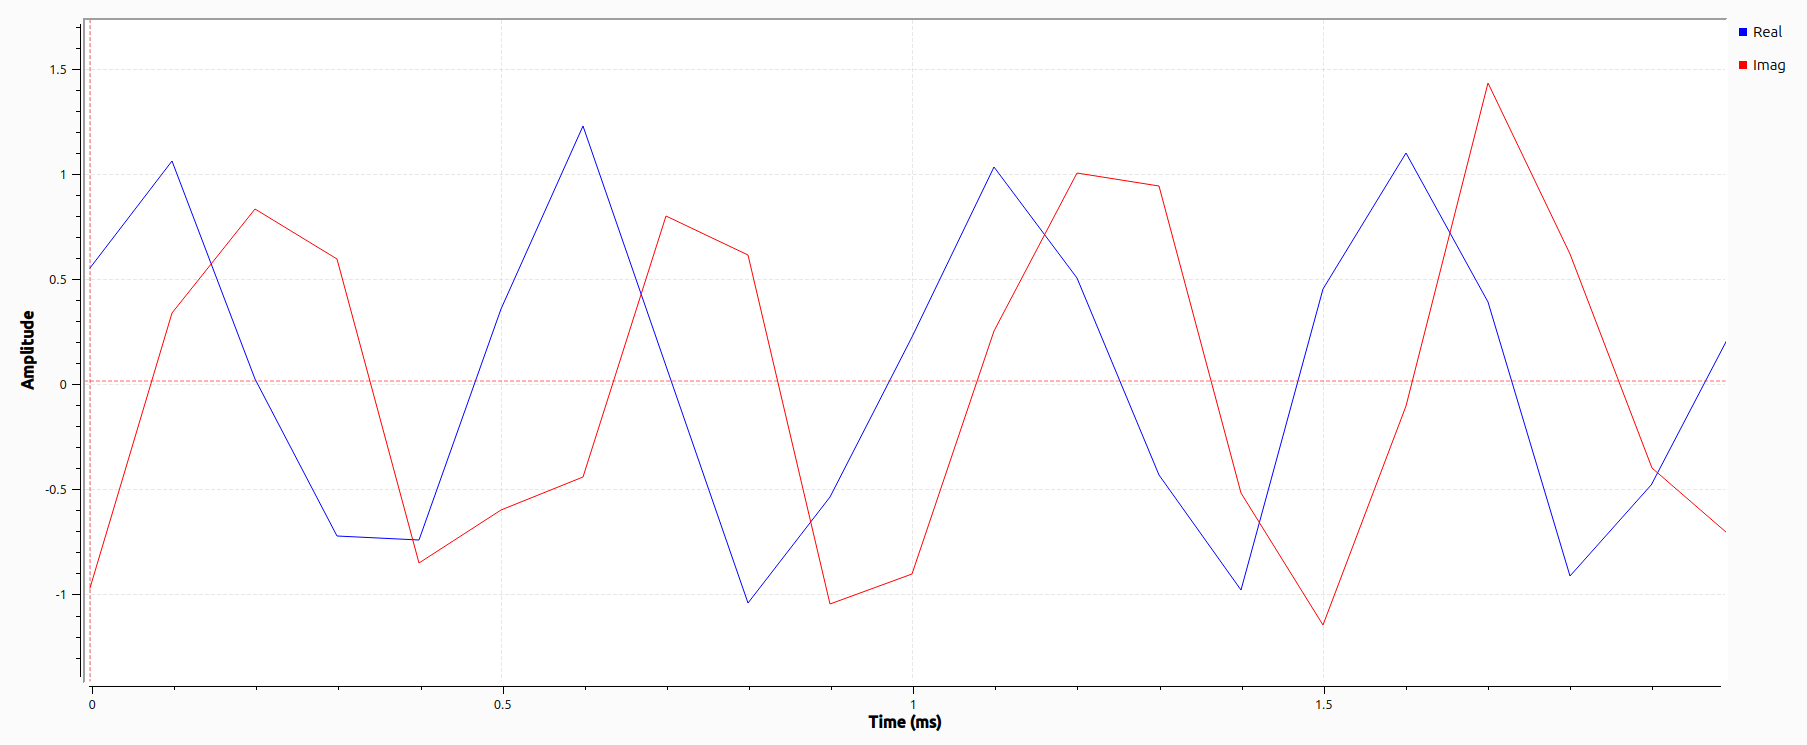
\includegraphics[width=0.7\textwidth]{noise_time_domain_10dB_snr.png}}}
	\caption{Time-Domain Sinusoid Data with AWGN Resulting in 10 dB SNR}
	\label{fig::noise_time_domain_10dB_snr}
\end{figure}

Comparing the above figure to Figure \ref{fig::sampling_rates_freq_domain_10k_samp_rate}, we see that the added noise randomizes the values of the peaks and zeros in the sampled data. With a low enough SNR, we could easily mask the sinusoid data with the noise. Figure \ref{fig::noise_freq_domain_20dB_snr} highlights the impact of AWGN on the frequency response.

\begin{figure}[H]
	\centerline{\fbox{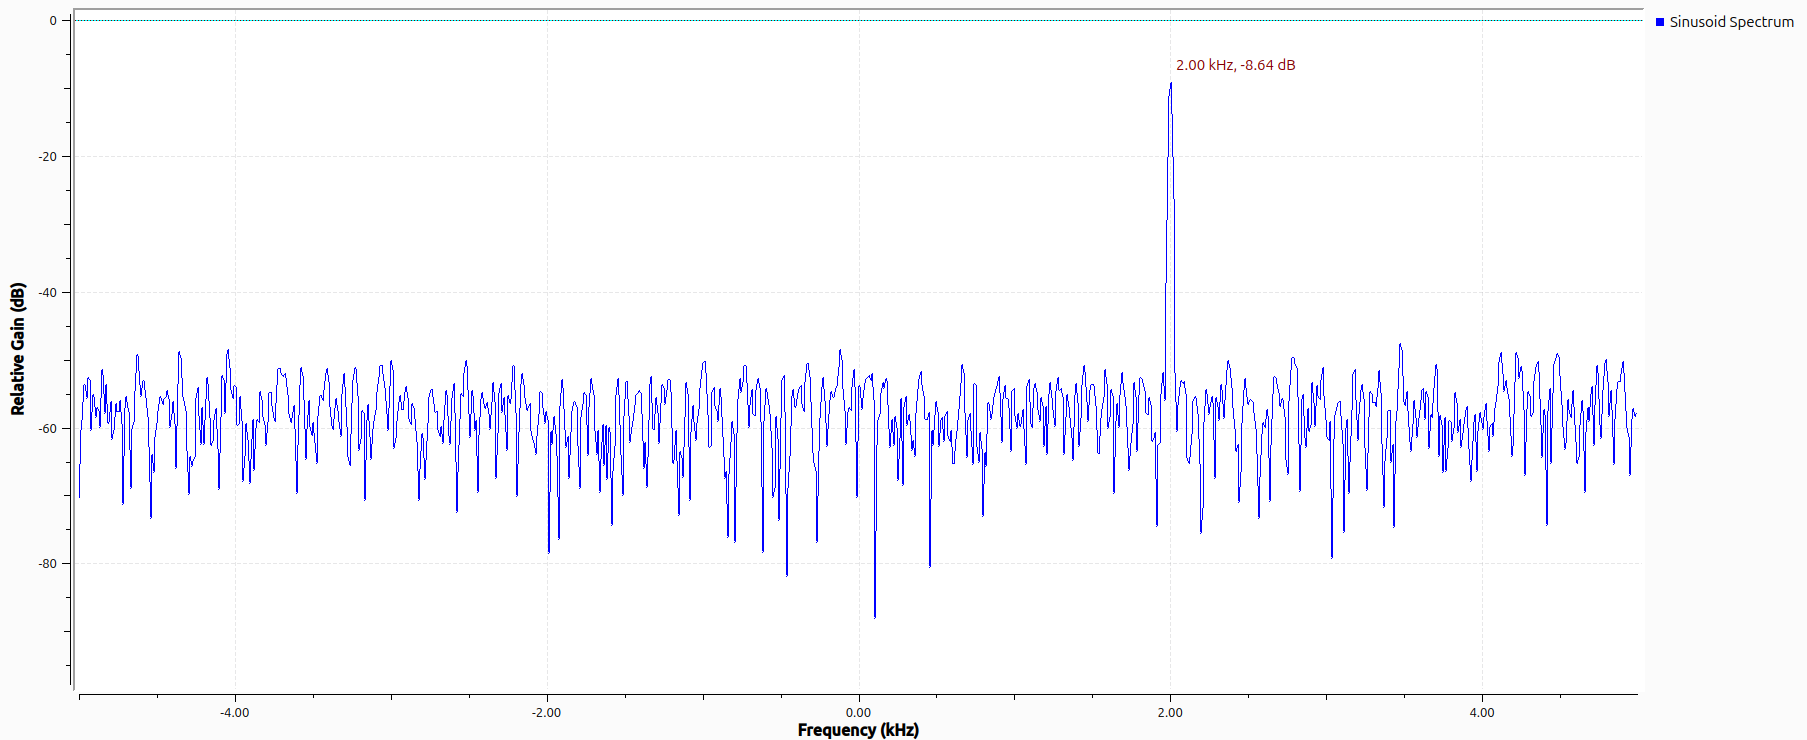
\includegraphics[width=0.7\textwidth]{noise_freq_domain_20dB_snr.png}}}
	\caption{Sinusoid Frequency Response with AWGN Resulting in 20 dB SNR}
	\label{fig::noise_freq_domain_20dB_snr}
\end{figure}

Comparing the above figure to Figure \ref{fig::sampling_rates_freq_domain_10k_samp_rate}, we see that the added noise has created a noise floor in the frequency response, well above the previously observed sidelobe levels. Figure \ref{fig::noise_constellation_20dB_snr} highlights the impact of AWGN noise on the received constellation.

\begin{figure}[H]
	\centerline{\fbox{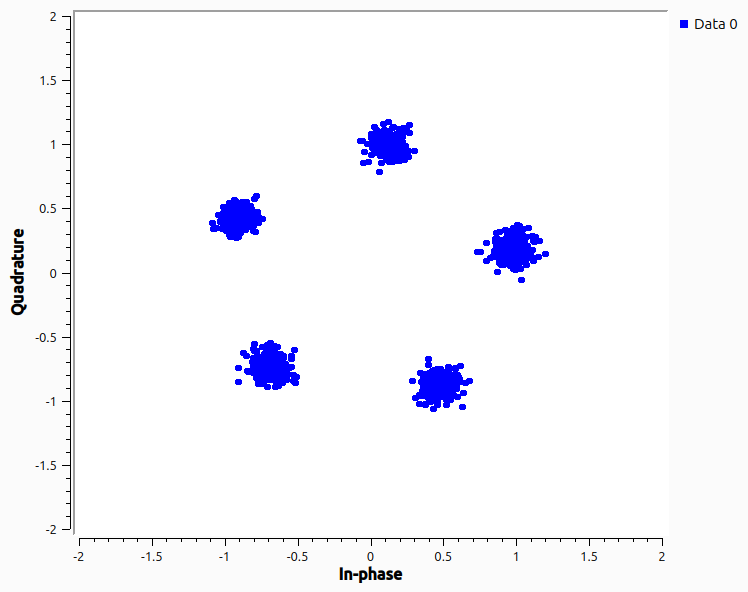
\includegraphics[width=0.7\textwidth]{noise_constellation_20dB_snr.png}}}
	\caption{Received Constellation with AWGN Resulting in 20 dB SNR}
	\label{fig::noise_constellation_20dB_snr}
\end{figure}

Comparing the above figure to Figure \ref{fig::iq_imbalance_0_mag_0_phase_10k_samp_rate_const}, the additive noise causes the expected constellation points to deviate from the expected constellation points. Luckily, at a 20 dB SNR, we can clearly distinguish which noise-free constellation point the data is associated with. Decreasing the SNR, increases the deviation between the constellation points and expected constellation points. This can lead to bit errors in a communication system which maps constellation points to sequences of bits.

We can also create histograms from the noise data to evaluate their pdf. Figure \ref{fig::gaussian_noise_histogram} shows the histogram of Guassian noise with an amplitude of 1. The resulting histogram is consistent with the bell-curve shape of the Gaussian pdf.

\begin{figure}[H]
	\centerline{\fbox{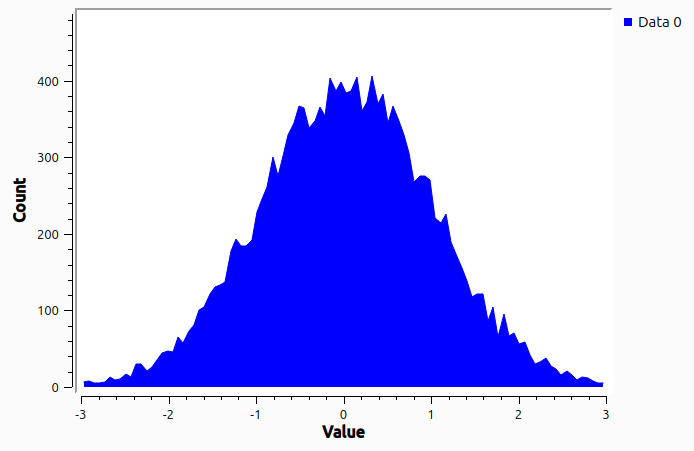
\includegraphics[width=0.7\textwidth]{gaussian_noise_histogram.png}}}
	\caption{Histogram of Guassian Noise Source with Amplitude of 1}
	\label{fig::gaussian_noise_histogram}
\end{figure}

Figure \ref{fig::uniform_noise_histogram} shows the histogram of Uniform noise with an amplitude of 1. The resulting histogram is consistent with the uniform pdf over the interval [-1,1).

\begin{figure}[H]
	\centerline{\fbox{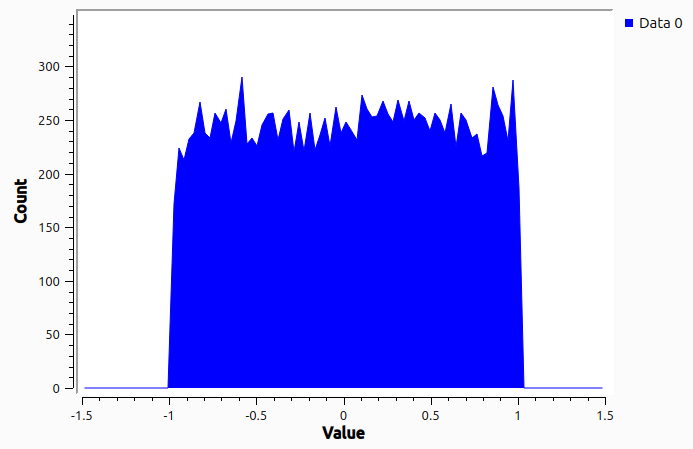
\includegraphics[width=0.7\textwidth]{uniform_noise_histogram.png}}}
	\caption{Histogram of Uniform Noise Source with Amplitude of 1}
	\label{fig::uniform_noise_histogram}
\end{figure}

Figure \ref{fig::laplacian_noise_histogram} shows the histogram of laplacian noise with an amplitude of 1. The resulting histogram highlights the exponential amplitude decay present in the laplacian pdf.

\begin{figure}[H]
	\centerline{\fbox{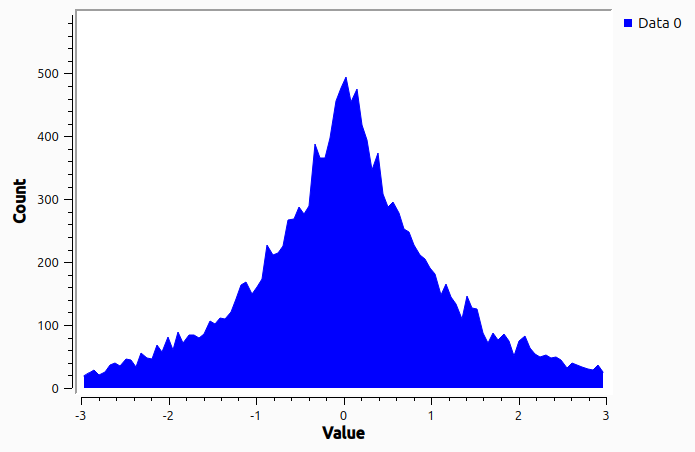
\includegraphics[width=0.7\textwidth]{laplacian_noise_histogram.png}}}
	\caption{Histogram of Laplacian Noise Source with Amplitude of 1}
	\label{fig::laplacian_noise_histogram}
\end{figure}

Figure \ref{fig::impulse_noise_histogram} shows the histogram of impulse noise with an amplitude of 1. Note that we only show a subset of the y-axis to better visualize the presence of high-amplitude impulse samples. The resulting histogram matches well with the pdf of impulse noise.

\begin{figure}[H]
	\centerline{\fbox{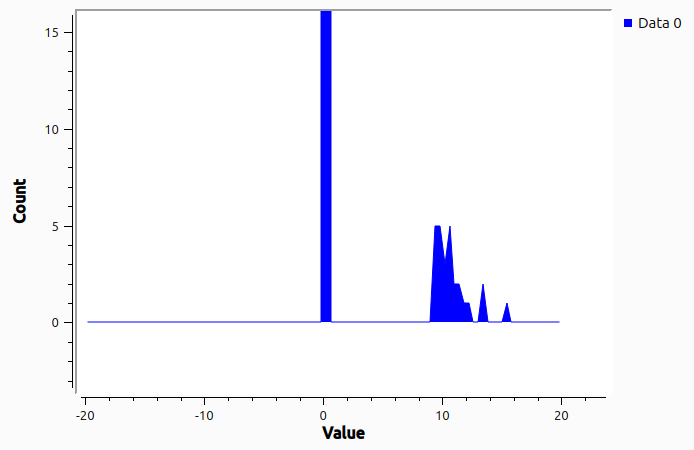
\includegraphics[width=0.7\textwidth]{impulse_noise_histogram.png}}}
	\caption{Histogram of Impulse Noise Source with Amplitude of 1}
	\label{fig::impulse_noise_histogram}
\end{figure}

\subsection{Interpolation and Decimation}

The final experiment we performed examined the impact of interpolation and decimation on the time and frequency-domain curves. Figure \ref{fig::interpolation_and_decimation_experiment} shows the setup for our examination, and Figure \ref{fig::interpolation_and_decimation_waveforms} shows the collected data. The top figure contains time-domain data and the bottom figure contains frequency-domain data. The blue waveform is the data before interpolation and decimation. The red data is the data interpolated by 4. And the green waveform is the data decimated by 4.

\begin{figure}[H]
	\centerline{\fbox{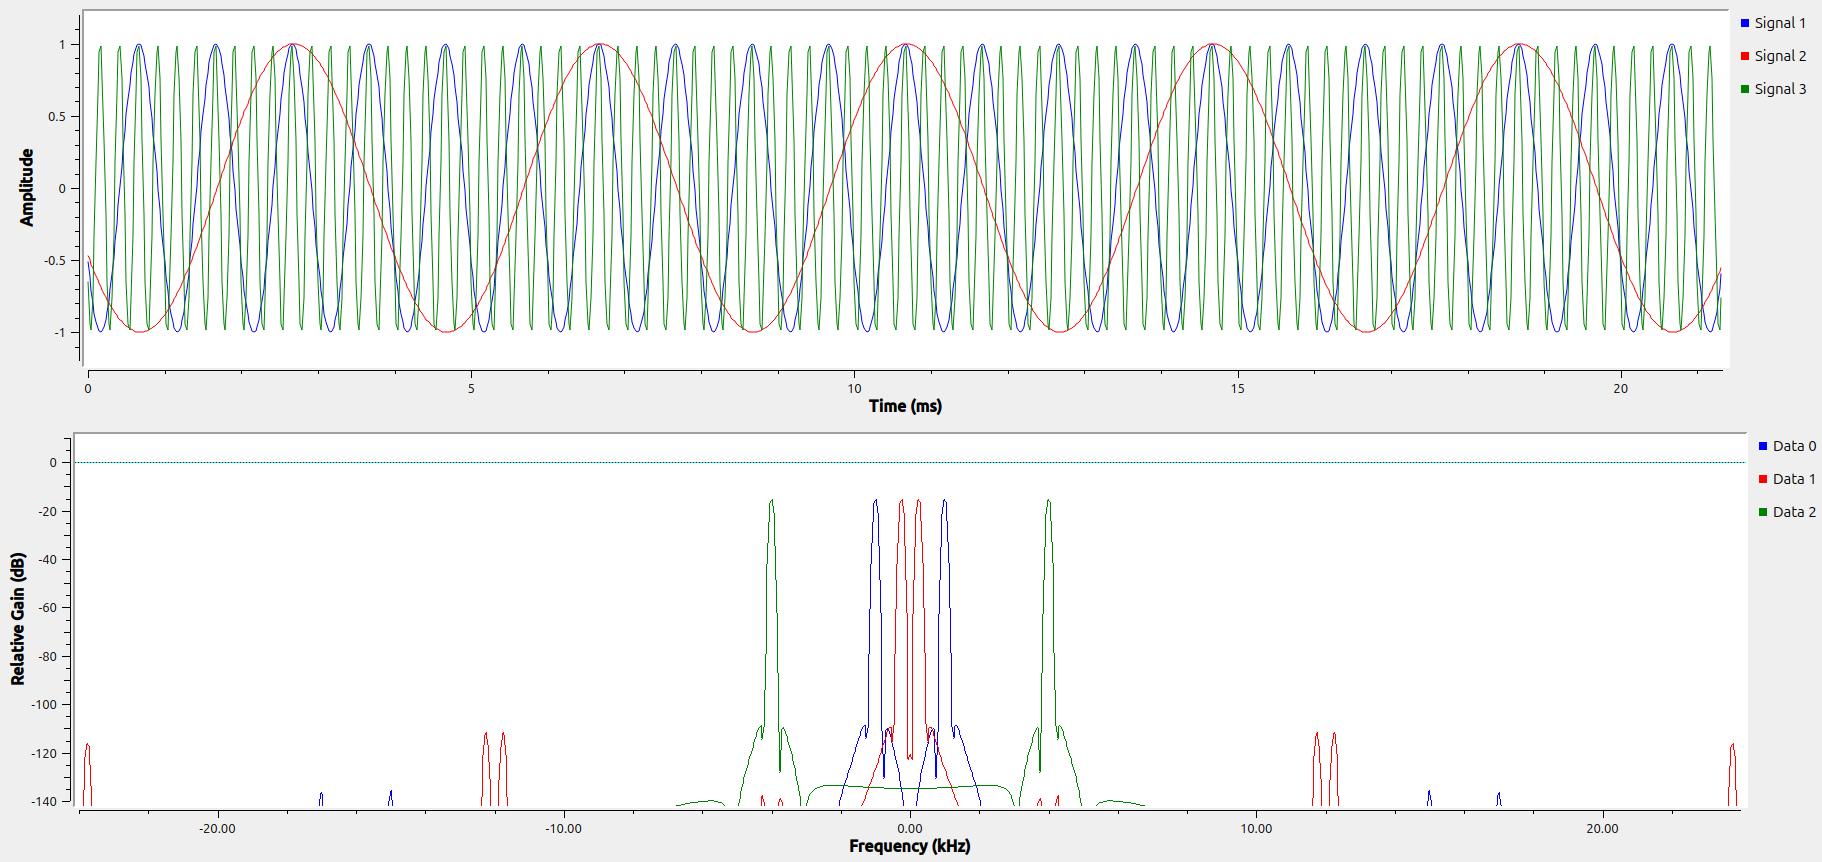
\includegraphics[width=0.7\textwidth]{interpolation_and_decimation_waveforms.png}}}
	\caption{Time and Frequency-Domain Data for Interpolated and Decimated Sinusoids}
	\label{fig::interpolation_and_decimation_waveforms}
\end{figure}

Each of the time-domain curves contains the same number of points plotted on a common x-axis. Therefore, the curve sampled at the highest rate contains the fewest number of sinusoid periods. The data in the frequency-domain curves is also plotted on a common x-axis. As a result, the displayed frequencies can be misleading. In the frequency-domain curves, the data sampled at the highest rate (interpolated data) will contain the largest span of frequency. Thus, the sinusoid peak frequencies will be closest to the origin. 

In the frequency response, the peaks of the interpolated data are 4x closer to the origin than the original data. When, we interpolate the data the spectral content is repeated 4x, and the spectral copies are filtered out. The filter is not perfect, so we see the spectral copies at a reduced power level. The peaks of the decimated data are 4x farther from the origin than the original data. When we decimate, the data is passed through an anti-aliasing filter prior to decimation. After filtering, whatever spectral content remains outside of $\pm\pi/4$ (normalized frequency) will alias on top of the remaining spectral content. Because we are sampling a perfect sinusoid, no spectral content will alias.

\subsection{Followup Questions}

\begin{enumerate}
	\item What are the benefits of using in-phase and quadrature (I \& Q) sampling in SDR? Fully describe at least three benefits of IQ sampling.
	
	IQ sampling eliminates the negative "ghost" frequencies from a real bandpass signal. IQ sampling also allows for baseband processing - significantly reducing the required sample rates (can sample at the bandwidth of the signal instead of at twice the highest frequency). Can sample at half of the rate of real signal-processing. Can perform coherent processing since we recover phase information.
	
	\item In GNU Radio What is the purpose of the Throttle block in GNU Radio? When should it be used? What happens if you use more than one throttle block? When is a throttle block unnecessary?

		The throttle block helps GNU radio avoid CPU congestion. Simulation will run as fast as the processor allows them to. If real-time scheduling is used, GNU radio could overtake CPU resources and crash the processor. The throttle block is unneeded if using hardware because the hardware provides flow control. When using hardware, the throttle block is unnecessary, redundant, and could add an undue bottleneck.
		
		Only need one element of flow control. Don't need to have multiple throttle block. Could even put throttle block in another spot of the flowchart and connect to null source/sink.
		
	\item  Explain Nyquist zones and their significance in software-defined radio.
	
	Nyquist zones are an artifact of the frequency wrapping that occurs when sampling. The Nyquist zones divide the spectrum into bands that are half the sampling rate. These bands are mirrored for the negative frequencies. Positive frequencies in odd nyquist zones wrap to positive frequencies in the 1st nyquist zone $[-f_s/2, f_s/2)$ and negative frequencies in odd nyquist zones wrap to negative frequencies in the 1st nyquist zone. The opposite relationship is true for even nyquist zones. (Positive frequencies wraps to negative frequencies, and negative frequencies wraps to positive frequencies). Traditional sampling (direct-conversion topology) assumes the signal is passed through a low pass filter and sampled in the first nyquist zone. However, we can also apply a bandpass filter to the signal and sample in different nyquist zones. In many systems, the required bandpass filter is already present for the conversion from RF to IF. We can directly sample the signal at IF at a sampling rate below the highest frequency as long as the signal is contained within a nyquist zone. This reduces the amount of analog hardware. This often done in heterodyne receivers, which replace the analog down-conversion stage with a digital down-conversion stage. This improves image rejection because there is no longer I/Q imbalance. However, the A/D bandwidth must be at least 2x that of a direct-conversion receiver because real sampling is used. As a result, this typology is limited to higher performing and more expensive SDRs.
	
	\item Why is dither noise added in Digital-to-Analog Converter (DAC) circuits?
	
	Dither is added to DAC circuits to increase the spur free dynamic range. Quantization of a continuous signal (especially sinusoids) can lead to large harmonics due to periodic errors in quantization. Dither noise helps to randomize the quantization error - reducing the amplitude of spurs.
	
\end{enumerate}



% The resulting figure is shown in Figure \ref{} and is identical to the Figure shown in \ref{fig}.



\section{Conclusion}
Conclusions to the overall lab that discuss meaningful lessons learned and other takeaways from the assignment. (Important)

%sampling rates
%complex samples
%interpolation
%decimation
%noise analysis

%\title{Lab 1 - Introduction to Software-Defined Radio\\
%
\includegraphics[scale=0.25\textwidth]{ua_logo.png}}
%\author{Owen Sowatzke}
%\date{\today}
%\maketitle

\end{document}